\chapter{Experimental Setup, and Evaluation Results}\label{Results_and_Discussion}
In this chapter, the experiments and results of the training and evaluation of the \gls{3d} shoe scan segmentation models are presented. Several experiments were conducted to analyze the performance and efficiency of different network configurations. The baseline model is the standard SegFormer architecture, which uses an \gls{mvt} as backbone. This model is compared against two alternative configurations: SegFormer with \gls{shvit} as backbone, and a modified version of SHViT: \gls{shvit_csa} that incorporates a central self-attention mechanism designed to improve spatial focus but also reduces memory consumption.

\medskip

\noindent The experiments are structured into five main parts:
\begin{enumerate}
	\item Backbone comparison: SegFormer with \gls{mvt}, \gls{shvit}, and \gls{shvit_csa} backbones are compared under various parameter settings. Model performance is evaluated using the F1-score as the primary accuracy metric, and \acrshort{gpu} memory consumption is reported to assess computational efficiency.
	
	\item Volume test: The maximum input volume size that can be processed by the \gls{shvit}-based model under hardware constraints is determined, revealing useful information about their scalability.
	
	\item Convolution layer depth: The number of convolutional layers in the \gls{shvit} head is varied, and its impact on segmentation performance (in terms of F1 but also voxel resolution) is analyzed.
	
	\item Kernel size analysis: The effect of varying kernel sizes in both the central self-attention mechanism and the attention block of the \gls{shvit} model is investigated to understand their influence on model accuracy.
	
	\item Direct comparison with literature: The segmentation performance of the proposed \gls{shvit}-based model is compared against existing approaches with \glspl{cnn} in the literature \cite{contribution_martin_leipert}. The evaluation focuses on benchmark metrics, particularly the F1-score for each segmented component on the same dataset, offering both qualitative and quantitative insights into how \gls{shvit} performs relative to \gls{cnn}-based methods.
\end{enumerate}

Together, these experiments aim to provide a comprehensive evaluation of transformer-based architectures for \gls{3d} volumetric segmentation of shoe scans, highlighting trade-offs between model complexity, accuracy, and computational requirements.

\medskip

For each configuration in the experiment, six independent training runs were performed to account for variability due to random initialization and data augmentation. From these six simulations, the best five (based on validation performance) were selected. The final reported F1-score for each configuration is the average of these five values. Error bars in the plots in the following sections represent the standard deviation across these best five runs, providing a measure of the model's stability and robustness.



\section[Backbone Comparison: MVT, SHViT, and SHViT with CSA]{Backbone Comparison: SegFormers with MVT, SHViT, and SHViT with Central Self-Attention}
The first experiment focuses on evaluating the impact of different backbone architectures on the segmentation performance of \gls{3d} shoe scans. As a baseline, the standard SegFormer model with an \gls{mvt} backbone is used. This backbone has shown strong performance in \gls{2d} semantic segmentation tasks \cite{xie2021segformersimpleefficientdesign} and serves as a reference point for comparison.

\medskip

To explore more efficient and potentially better-suited alternatives for volumetric data, the \gls{mvt} backbone is replaced with \gls{shvit}, which is designed to better capture spatial dependencies in \gls{3d} data while maintaining computational efficiency. Furthermore, a modified version of \gls{shvit} is introduced, in which the conventional self-attention mechanism is replaced with a central self-attention block. This modification aims to enhance local spatial sensitivity and improve segmentation quality, particularly in regions with fine-grained structural details, but also helps to reduce memory consumption.

\medskip

All models in this experiment use a fixed input volume size of {\tt (224,224,224)} voxels and a segmentation output size of {\tt (56,56,56)}, determined by the number of downsampling steps and convolutional layers. Specifically, a two-layer convolutional encoder head is used across all configurations to map the feature representations to the final segmentation mask. Larger volumes such as {\tt (256,256,256)} exceed the available \acrshort{gpu} memory of 24\,GB when using the \gls{shvit} backbone with the B5/S4 configuration, and a fair comparison would not be possible.

\medskip

Each of these backbone configurations is tested using various hyperparameter settings to assess their robustness and performance under different conditions. The models are evaluated based on their segmentation accuracy, measured using the F1, their \acrshort{gpu} memory consumption, and the number of trainable parameters. This comparison illustrates the trade-offs between model complexity, resource requirements, and segmentation quality when applying transformer-based architectures to \gls{3d} imaging data.

\bigskip

Figure \ref{iou_vs_gpu_memory} shows a plot of F1-score versus \acrshort{gpu} memory consumption for the different backbone architectures and parameter configurations. Three distinct accuracy levels can be observed in the plot. 
\begin{figure}[H]
	\centering
	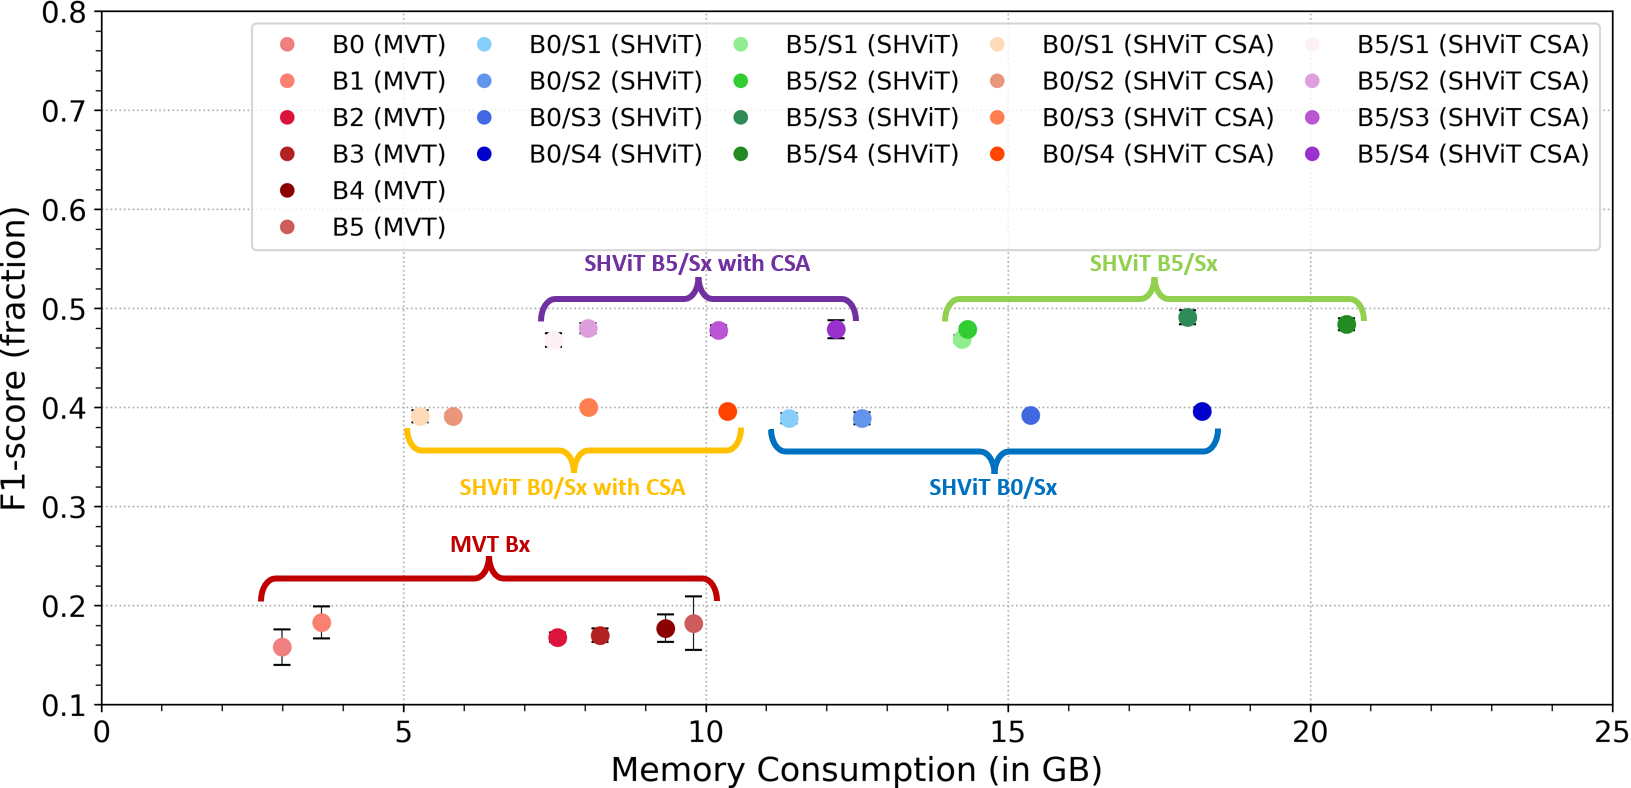
\includegraphics[width=1.0\textwidth]{./images/F1_vs_gpu_memory_w_text.png}
	\caption[F1-score versus GPU memory consumption]{F1-score versus GPU memory consumption for different parameter sets for MVT, SHViT, and SHViT with central self-attention (CSA)}
	\label{iou_vs_gpu_memory}
\end{figure}
The lowest group, with F1 values between 0.1 and  0.2, corresponds to models using the \gls{mvt} backbone, indicating limited segmentation performance on the \gls{3d} shoe scan task. The second group, with F1-score around 0.4, results from experiments using the \gls{shvit} backbone with the B0/Sx\footnote{see table \ref{tab:variants} on page \pageref{tab:variants}.} parameter settings, demonstrating improved accuracy compared to \gls{mvt} while maintaining relatively low memory usage. The highest accuracy group, with F1 values slightly below 0.5, is achieved using \gls{shvit} with the B5/Sx configuration, suggesting that deeper and more expressive backbone variants lead to significantly better segmentation performance, but this comes with increased memory consumption.

\medskip

While the standard \gls{shvit} models already outperform \gls{mvt} in terms of accuracy, they tend to consume more \acrshort{gpu} memory. However, introducing the central self-attention mechanism significantly reduces memory usage between 43\% and 54\% (for B0/Sx-configurations) and between 41\% and 47\% (for B5/Sx) without compromising segmentation performance. This highlights the central self-attention variant as a more efficient alternative, offering a favorable trade-off between computational cost and predictive accuracy.

\medskip

An intriguing observation from the experiment is the differing sensitivity of the two backbone types to their respective hyperparameter settings. For the standard SegFormer model with the \gls{mvt} backbone, the F1 accuracy improves noticeably when progressing from the B0 to the B5 configuration. This indicates that increasing model capacity through deeper and wider transformer layers positively impacts segmentation performance. In contrast, the \gls{shvit}-based models show relatively stable F1 performance across the different Sx configurations (S1 to S4), regardless of whether B0 or B5 decoding dimensions are used. This suggests that the \gls{shvit} backbone is less sensitive to internal architectural scaling and that even its smaller configurations are able to extract meaningful features from the \gls{3d} volumes effectively.

\medskip

It was initially expected that the \gls{mvt}-based SegFormer model would achieve significantly better results on the \gls{3d} shoe scan data, given its strong performance on \gls{2d} segmentation benchmarks. In \gls{2d} experiments, the \gls{mvt} backbone consistently produced high \gls{iou} values \cite{xie2021segformersimpleefficientdesign}. However, in this study, the \gls{mvt} model performed notably worse on the volumetric data, achieving only small \gls{iou} scores with 0.2 and below\footnote{For this comparison the \gls{iou} was also calculated.}. This performance gap suggests that while the \gls{mvt} architecture is well-suited for \gls{2d} spatial relationships, it does not generalize effectively to \gls{3d} volumetric data without further architectural adaptations.

\bigskip

Another noteworthy observation is the significant difference in the number of trainable parameters between the \gls{mvt}-based and \gls{shvit}-based models, as shown in figure \ref{iou_vs_train_parameters}. For the \gls{mvt} backbone, the number of parameters spans a wide range, from approximately 5 million in the B0 configuration up to around 120 million for B5. In contrast, all \gls{shvit}-based models, including those augmented with central self-attention, remain significantly more compact, with a maximum of approximately 20 million trainable parameters. This big decrease in model size shows the efficiency of the \gls{shvit} architecture, which achieves comparable or superior segmentation performance while maintaining a much lower parameter count, making it particularly attractive for resource-constrained environments.
\begin{figure}[H]
	\centering
	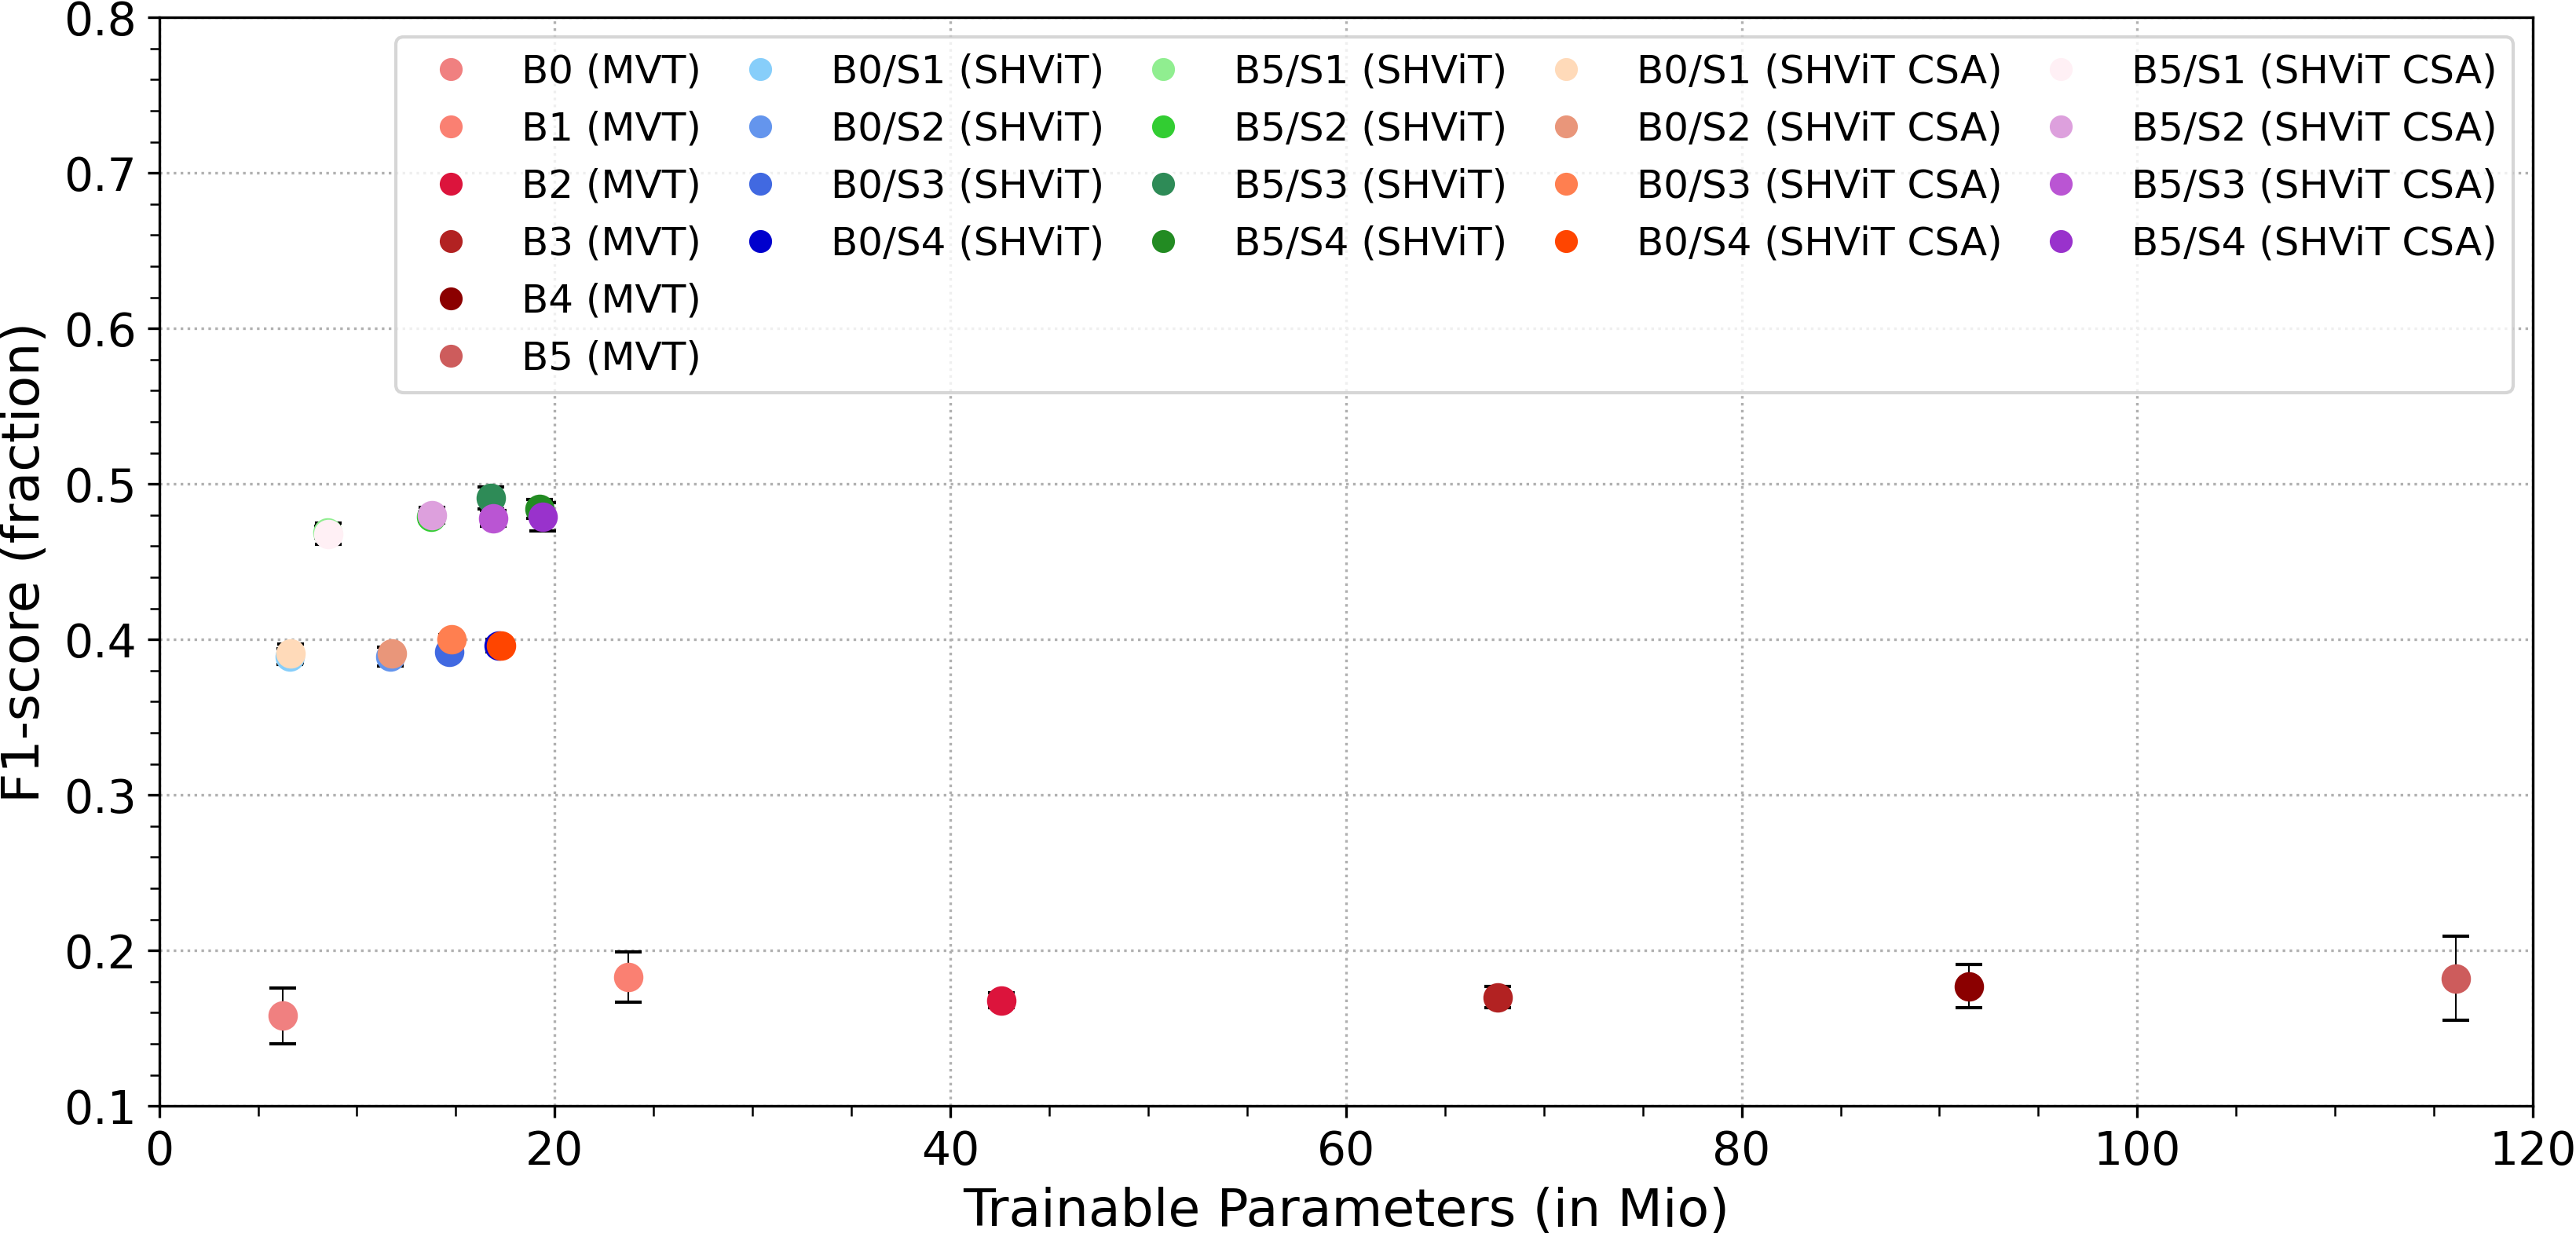
\includegraphics[width=1.0\textwidth]{./images/F1_vs_train_parameters.png}
	\caption[F1-score versus number of trainable parameters]{F1-score versus number of trainable parameters for different parameter sets for MVT, SHViT, and SHViT with central self-attention (CSA)}
	\label{iou_vs_train_parameters}
\end{figure}

Some results of the trained segmentation model on selected shoe volumes are shown in figure \ref{result_for_shvit_with_center_attention} for the \gls{shvit}-model with central self-attention and input volume size of {\tt (224,224,224)}. For each case, a central slice of the \gls{3d} volume is displayed, showing from left to right: the input image, the predicted segmentation, and the corresponding ground truth. These examples illustrate the model's performance in identifying and segmenting the relevant components within the shoe scans.

\medskip

For the subsequent experiments, the \gls{shvit} model with central self-attention and the B5/S2\footnote{see table \ref{tab:variants} on page \pageref{tab:variants}.} configuration was selected, as it provides a favorable balance between segmentation accuracy and memory efficiency in the initial comparison.

\begin{figure}[H]
	\centering
%	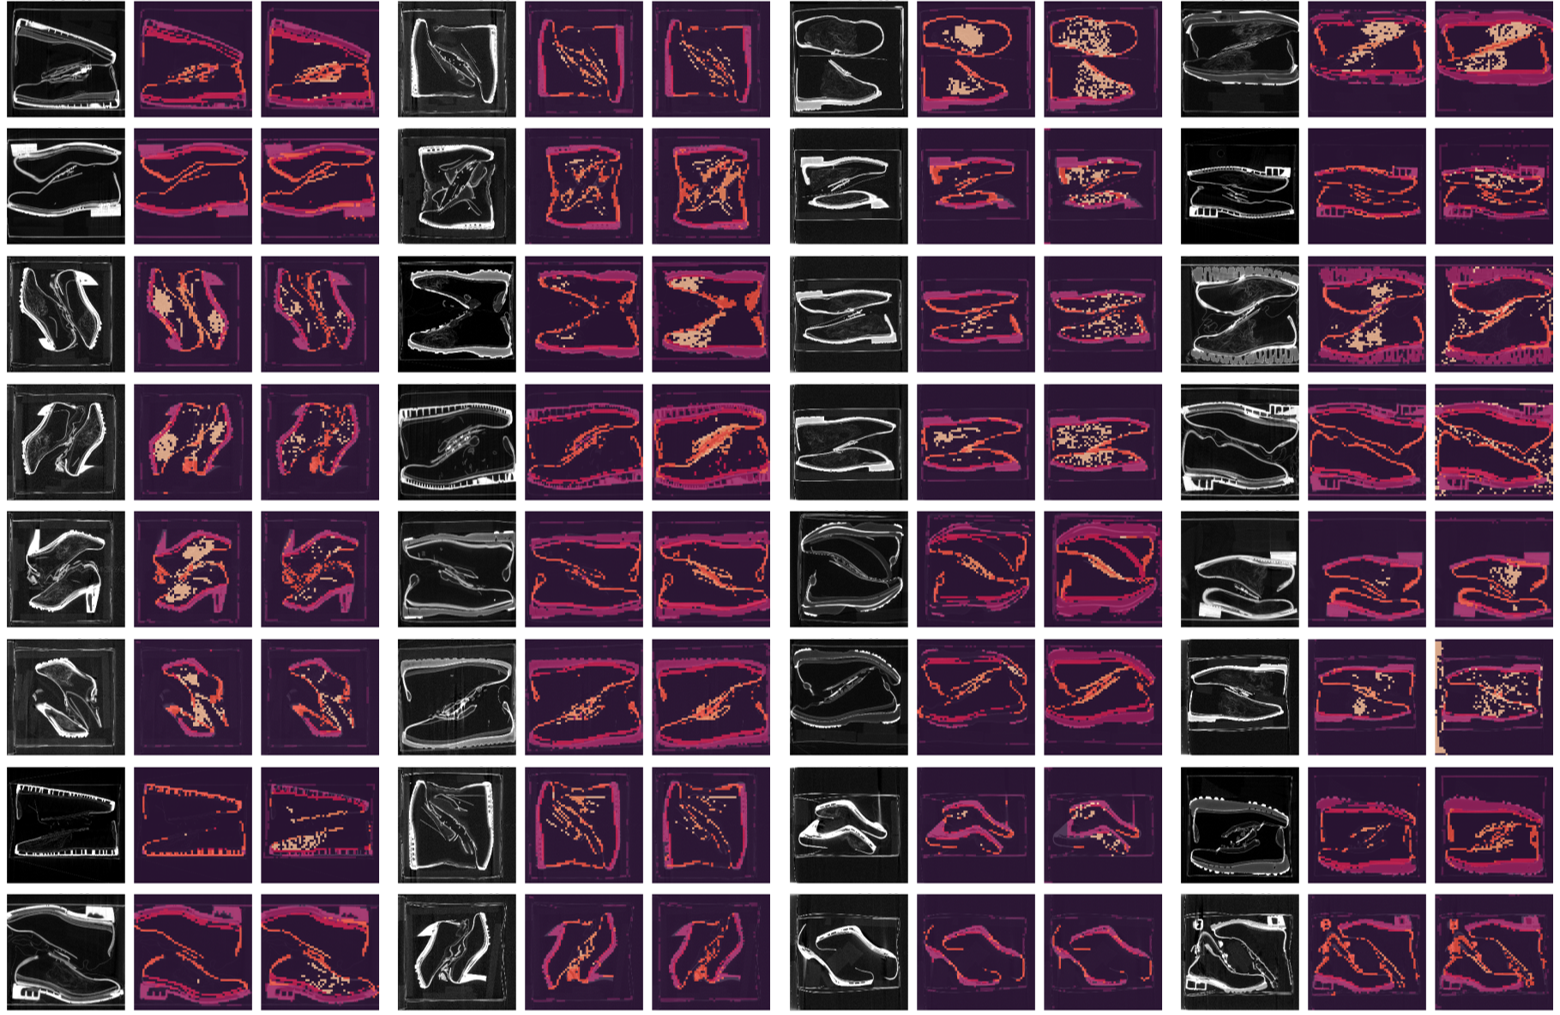
\includegraphics[width=1.0\textwidth]{./images/Shoes_224x224x224_B5S2.png}
%	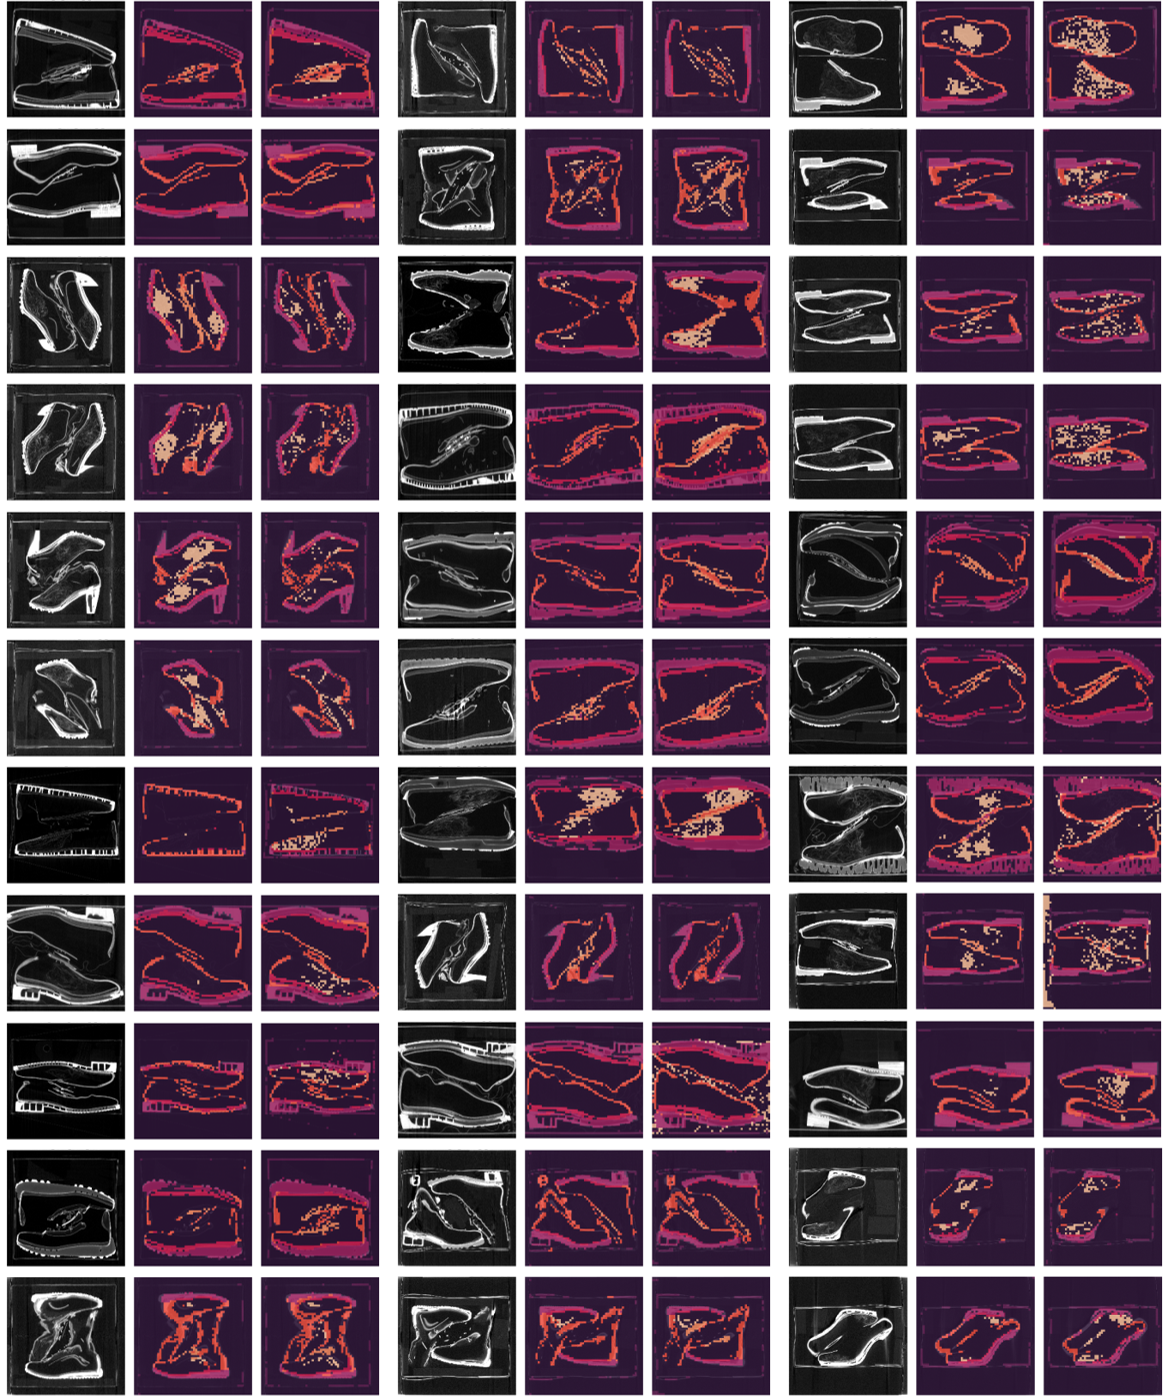
\includegraphics[width=1.0\textwidth]{./images/Shoes_224x224x224_B5S2_v2.png}
	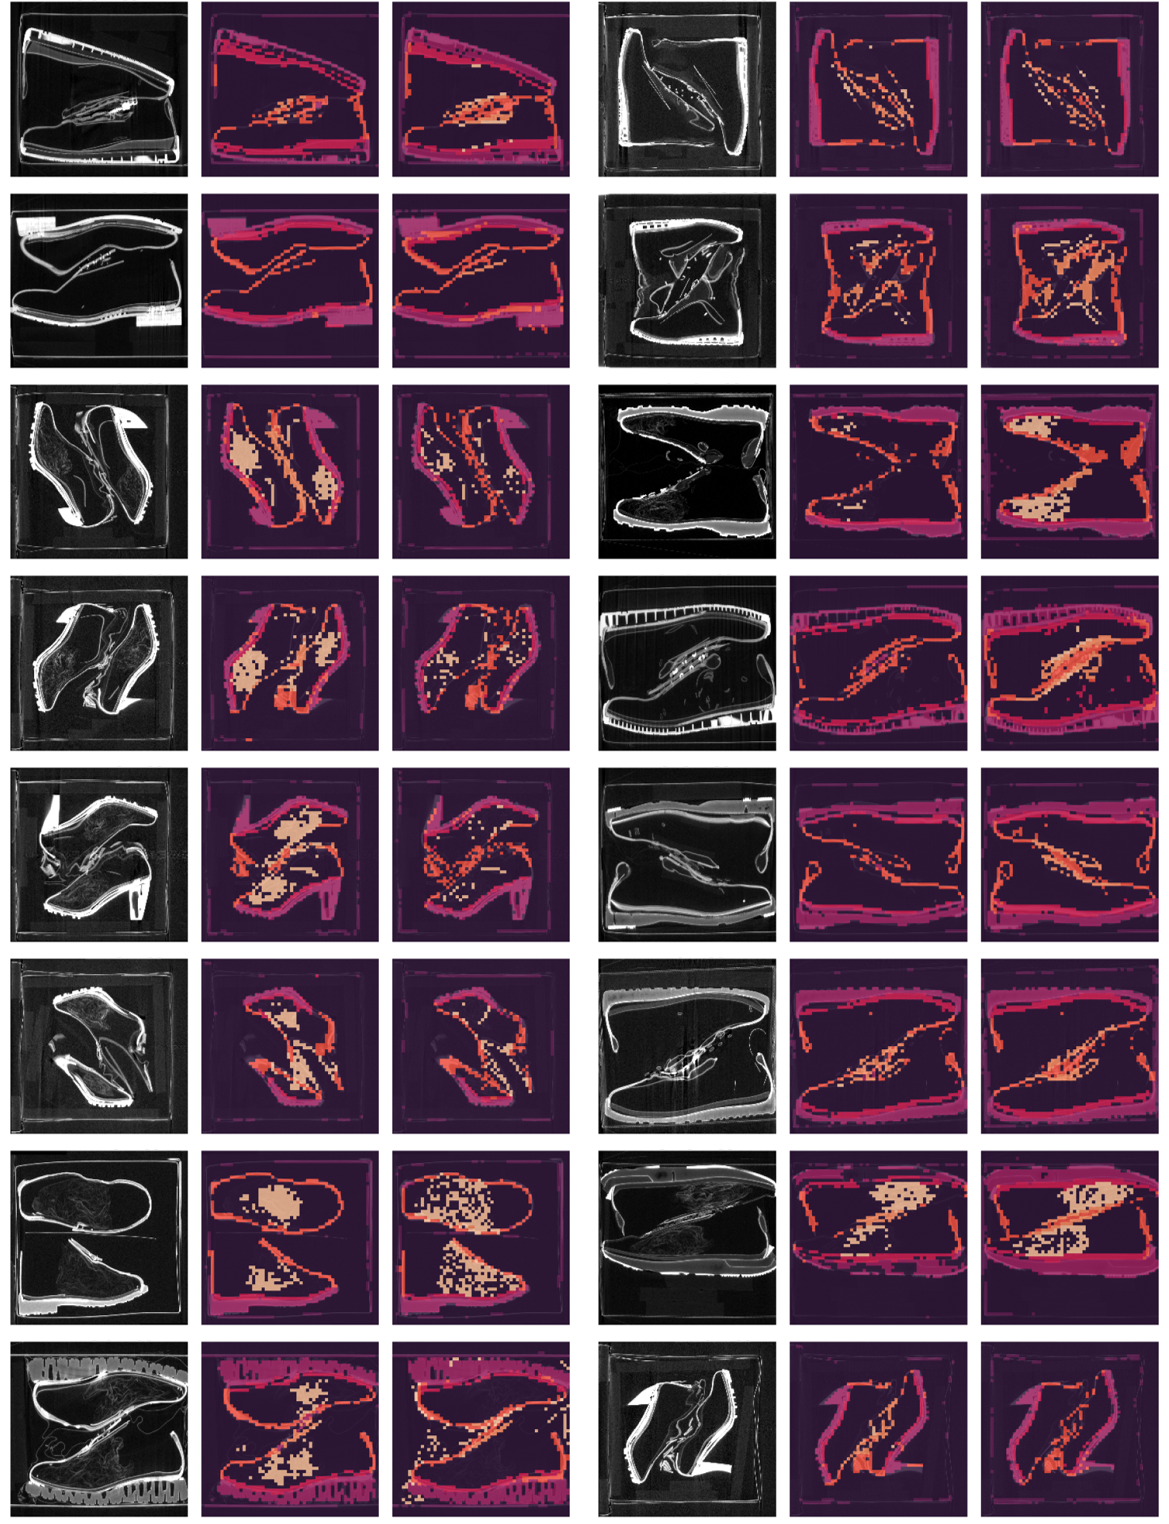
\includegraphics[width=1.0\textwidth]{./images/Shoes_224x224x224_B5S2_v3.png}
	
\includegraphics[width=0.9925\textwidth]{./images/color_legend_7_classes.png}
	\caption[Results of some shoes trained with the 3D-SHViT model with central self-attention]{Results of some shoes trained with the 3D-SHViT model with central self-attention. From left to right: the input image, the predicted segmentation, and the corresponding ground truth segmentation image for each of the two columns.}
	\label{result_for_shvit_with_center_attention}
\end{figure}



\section{Evaluation of Maximum Volume Size for SHViT on a 24\,GB GPU}
The second experiment aims to determine the maximum input volume size that can be processed by \gls{shvit}-based models under given hardware limitations. Understanding the scalability of the architecture is crucial for real-world applications, where high-resolution volumetric data is often desirable but constrained by \acrshort{gpu} memory capacity.

\medskip

By systematically increasing the input dimensions while monitoring memory usage, this analysis identifies the practical upper bounds for volume size on a 24\,GB \acrshort{gpu}. The results provide valuable insights into the efficiency of the \gls{shvit} architecture and its suitability for processing large-scale \gls{3d} inputs, especially in comparison to more memory-intensive transformer backbones.

\medskip

As demonstrated in the previous section, the \gls{shvit} model with central self-attention outperforms the other configurations in terms of segmentation accuracy and memory efficiency. Therefore, this model configuration is selected for the subsequent experiment to further explore its performance with different volume sizes.

\medskip

Figure \ref{iou_vs_vol_memory} shows the relationship between F1-score and \acrshort{gpu} memory consumption for different input volume sizes from the \gls{shvit} B5/S2-model. It can be observed that for very small volumes (e.g., {\tt (96,96,96)}, the F1-score is with 0.375 relatively low. As the volume size increases, the F1-score improves until it reaches a plateau at a volume size of {\tt (256,256,256)}. After this point, the F1-score remains flat, with only a very slight increase observed starting from a volume size of {\tt (320,320,320)}. The volume size of {\tt (352,352,352)} was not tested due to memory limitations, as it would have increased \gls{gpu}-memory usage to approximately 54\,GB.

\medskip

The lower F1-score at a volume size of {\tt (96,96,96)} may be attributed to both the lower resolution of the input volume and the relatively small size of the segment volume, which has a resolution of {\tt (24,24,24)}. This small segment volume limits the ability to capture fine details. As the input volume increases, the segment volume increases as well, leading to better performance. Table \ref{tab:volume_stages} illustrates the volume sizes at each stage of the \gls{shvit} model with 2 convolution layers in \gls{shvit} head, which already reduces the input size by a factor of 4.
\begin{figure}[H]
	\centering
	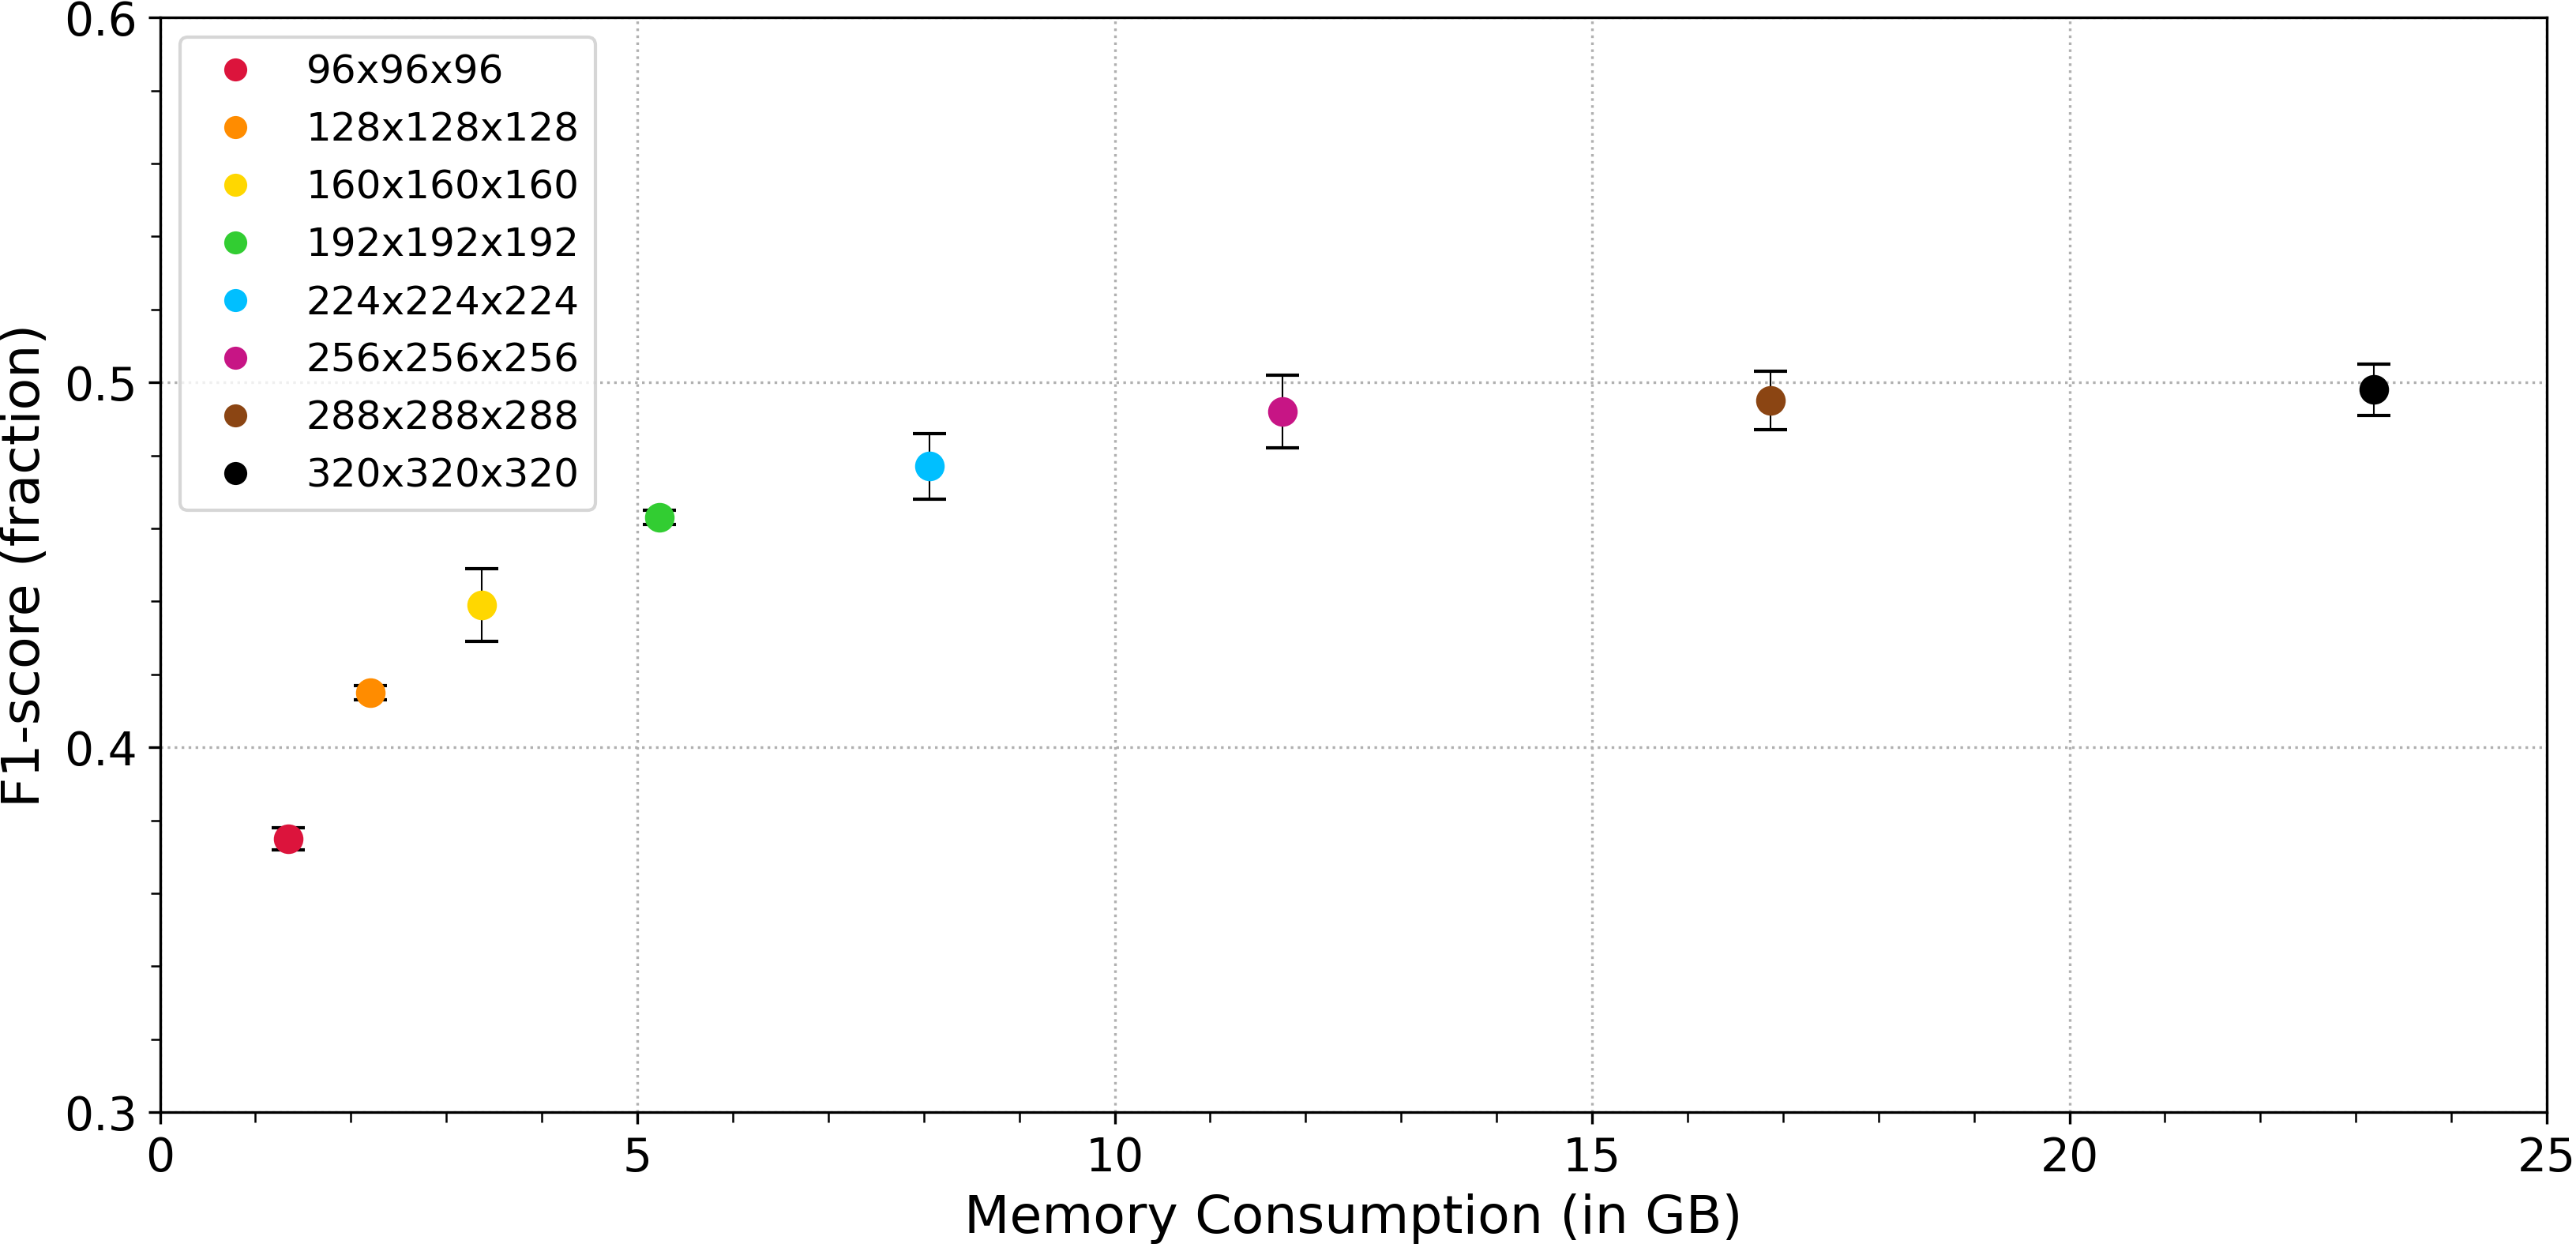
\includegraphics[width=1.0\textwidth]{./images/F1_vs_vol_memory.png}
	\caption[F1-score versus GPU memory consumption for different volume sizes]{F1-score versus GPU memory consumption for different volume sizes. The base model is SHViT B5/S2 with central self-attention.}
	\label{iou_vs_vol_memory}
\end{figure}

\begin{center}
\begin{threeparttable}[H]
	\begin{tabular}{c|cccc|c|c}
		\toprule
		\CellWithForcedBreak{volume \\ input \\ size} & \CellWithForcedBreak{size before \\ 1st stage} & \CellWithForcedBreak{size before \\ 2nd stage} & \CellWithForcedBreak{size before \\ 3rd stage} & \CellWithForcedBreak{size after \\ 3rd stage} & \CellWithForcedBreak{segment \\ volume \\ size} & \CellWithForcedBreak{max. \\ memory \\ consumption} \\
		\midrule
		\midrule
		96 & 24 & 24 & 12 &  6 & 24 & 1.34\,GB \\
		128 & 32 & 32 & 16 &  8 & 32 & 2.20\,GB \\
		160 & 40 & 40 & 20 &  10 & 40 & 3.37\,GB \\
		192 & 48 & 48 & 24 &  12 & 48 & 5.23\,GB \\
		{\bf 224} & {\bf 56} & {\bf 56} & {\bf 28} &  {\bf 14} & {\bf 56} & {\bf 8.05\,GB} \\
		256 & 64 & 64 & 32 &  16 & 64 & 11.76\,GB \\
		288 & 72 & 72 & 36 &  18 & 72 & 16.87\,GB \\
		320 & 80 & 80 & 40 & 20 & 80 & 23.19\,GB \\
		\midrule
		352 & 88 & 88 & 44 & 22 & 88 & >50\,GB \\
		\bottomrule
	\end{tabular}
	\caption[Overview of input volume sizes and their corresponding resolutions after each stage of the SHViT B5/S2-model]{Overview of input volume sizes and their corresponding resolutions after each stage of the SHViT B5/S2-model. The input volume is progressively reduced by convolutional layers (each with a stride of 2), and the resulting resolutions before/after each stage are shown. Between each stage is also a downsampling layer which reduces the volume by a factor of 2 (see figure \ref{Architecture_of_SHViT_Segformer} for details). The final segmentation volume is constructed from the outputs in the SegFormer decoder of the three stages of SHViT.}
	\label{tab:volume_stages}	
\end{threeparttable}
\end{center}

It is important to note that the segment output is derived from the last three stages of the \gls{shvit} model, meaning the input volume size of the first stage dictates the size of the segment output. Furthermore, not all volume sizes are feasible due to the structure of the model. After each stage, a convolution layer reduces the volume size by a factor of 2. Therefore, the output size at each stage should always be even (except for the last stage where it could also be uneven), as the upsampling in the \gls{mlp} layer and subsequent concatenation with previous layers require matching dimensions.

\medskip

Figure \ref{comparison_segmentations_for_different_volume_sizes} shows the predicted segmentation images for three different input volume sizes.

\begin{figure}[H]
	\centering
	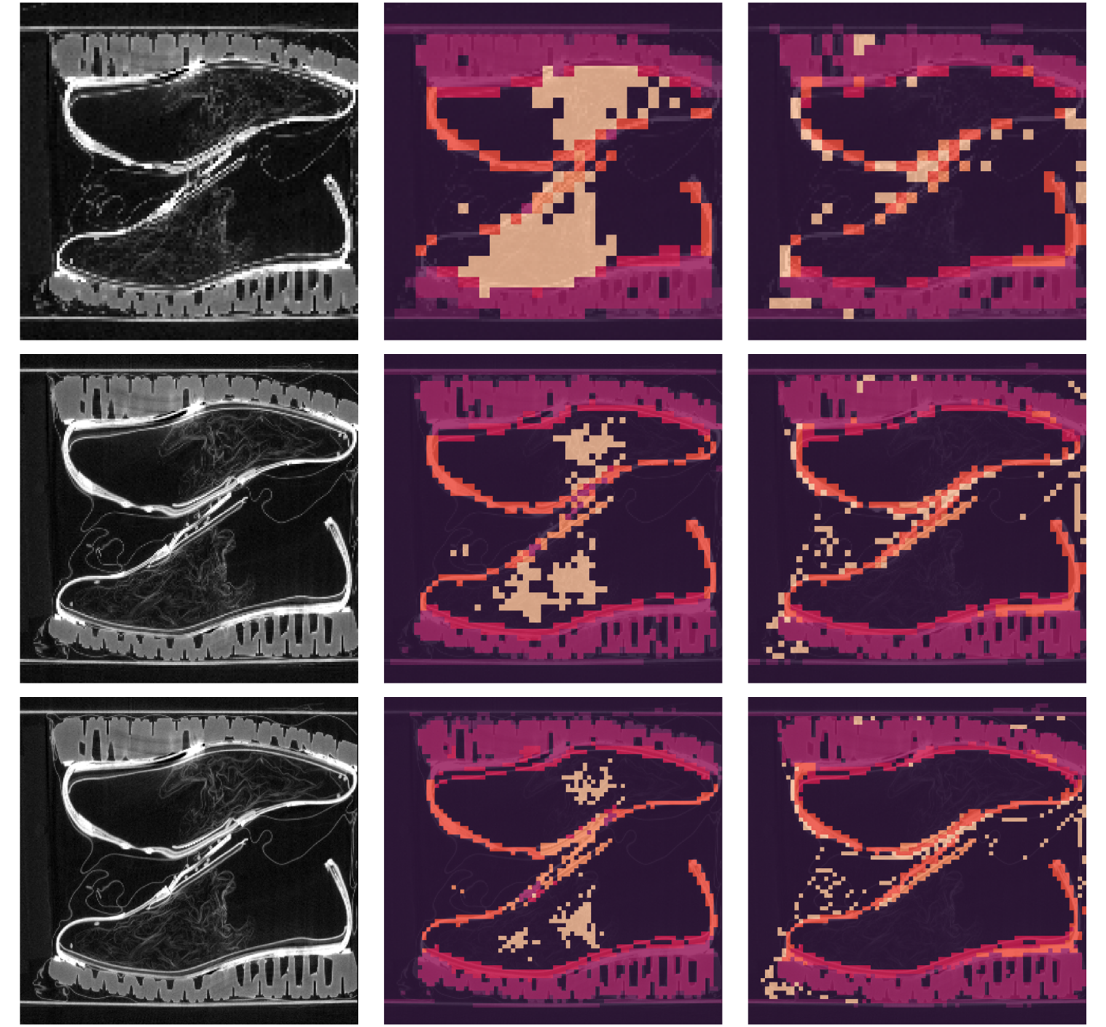
\includegraphics[width=0.7\textwidth]{./images/Shoepassion_40_down2_2_2_128-224-320.png}
	
\includegraphics[width=0.8\textwidth]{./images/color_legend_7_classes_v2.png}
	\caption[Comparison of the results with different volume sizes]{Comparison of the results with different volume sizes for {\tt Shoepassion\_40\_down2\_2\_2}. From left to right: the input image, the predicted segmentation, and the corresponding ground truth segmentation image. From top to bottom: input sizes increase from {\tt (128,128,128)} to {\tt (224,224,224)} and {\tt (320,320,320)}, with corresponding segmentation sizes from {\tt (32,32,32)} to {\tt (56,56,56)} and {\tt (80,80,80)}. For this pair of shoes, the predicted segmentation includes the filling material (visible inside the shoe), which is absent in the ground truth image, pointing to a potential inconsistency or omission in the labeling of this particular instance.}
	\label{comparison_segmentations_for_different_volume_sizes}
\end{figure}

The visualizations demonstrate how the resolution of the segmentation output varies with the input size. In particular, the coarseness of the segmentation at lower resolutions becomes evident, highlighting the limitations of small input volumes in accurately capturing fine structural details.


\section{Impact of Convolutional Depth on F1-score}
In this section, the influence of the number of convolutional layers $N$ in the \gls{shvit} segmentation head (overlay patch embedding, see figure \ref{Architecture_of_SHViT}) on both segmentation accuracy and \acrshort{gpu} memory consumption is analyzed. The convolutional layers in the head are responsible for processing the output features from the backbone and generating the final segmentation volume. By adjusting the depth of these layers, the trade-off between model complexity, segmentation quality (measured by F1-score), and computational efficiency is explored. 

\medskip

Each convolutional layer in the \gls{shvit} head reduces the spatial dimensions of the input by a factor of 2 due to the use of a stride of 2. Consequently, the output shape after $N$ convolutional layers can be calculated using the following formula:
\begin{equation}
\text{Output Shape} = \left(\frac{D}{2^N},\frac{H}{2^N},\frac{W}{2^N}\right)
\end{equation}
where $D$, $H$, and $W$ represent the depth, height, and width of the input volume, respectively, and $N$ is the number of convolutional layers. This relationship is essential for selecting compatible input sizes and ensuring consistent output dimensions across experiments.

\medskip

For this experiment, only those configurations of the \gls{shvit} head were evaluated that were feasible within available 24\,GB \acrshort{gpu} memory limits. Specifically, three variants with 1, 2, and 3 convolutional layers were tested\footnote{In addition to the high \acrshort{gpu} memory consumption associated with using 4 convolutional layers and a large input volume, the resulting file size per shoe amounts to approximately 2.7\,GB. This significantly increases the computational burden, not only in terms of memory usage but also in terms of training time, as the large volume files must be read from the \acrshort{ssd} for each epoch. This I/O overhead further limits the practicality of such configurations in resource-constrained environments.}. To ensure fair comparison across all configurations, the input volume size was adjusted so that the resulting segmentation output size remained constant at {\tt (56,56,56)}. This design choice eliminates potential confounding effects caused by differing output resolutions and enables a focused analysis of how convolutional depth influences segmentation performance and memory usage. Table~\ref{tab:volume_layers} summarizes the evaluated setups.

\begin{center}
	\begin{threeparttable}[H]
		\begin{tabular}{c|c|c|c|c}
			\toprule
			\CellWithForcedBreak{number of \\ conv layers N} & \CellWithForcedBreak{volume \\ input size} & \CellWithForcedBreak{size after \\ N conv layers} & \CellWithForcedBreak{segment \\ volume size} & \CellWithForcedBreak{max. memory \\ consumption} \\
			\midrule
			\midrule
			1 & 112 & 56 & 56 & 7.62\,GB \\
			{\bf 2} & {\bf 224} & {\bf 56} & {\bf 56} & {\bf 8.05\,GB} \\
			3 & 448 & 56 & 56 & 13.07\,GB \\
			\midrule
			4 & 896 & 56 & 56 & >50\,GB \\
			\bottomrule
		\end{tabular}
		\caption[Overview of input volume sizes and their corresponding segmentation resolutions of the SHViT B5/S2-model for different numbers of conv.~layers]{Overview of input volume sizes and their corresponding segmentation resolutions of the SHViT B5/S2-model for different numbers of convolutional layers.}
		\label{tab:volume_layers}
	\end{threeparttable}
\end{center}

The following figure \ref{iou_vs_layers_memory} illustrates the relationship between F1-score and \acrshort{gpu} memory consumption for three different \gls{shvit} head configurations. The configuration with only one convolutional layer gives the lowest accuracy, likely due to the reduced input resolution. 
\begin{figure}[H]
	\centering
	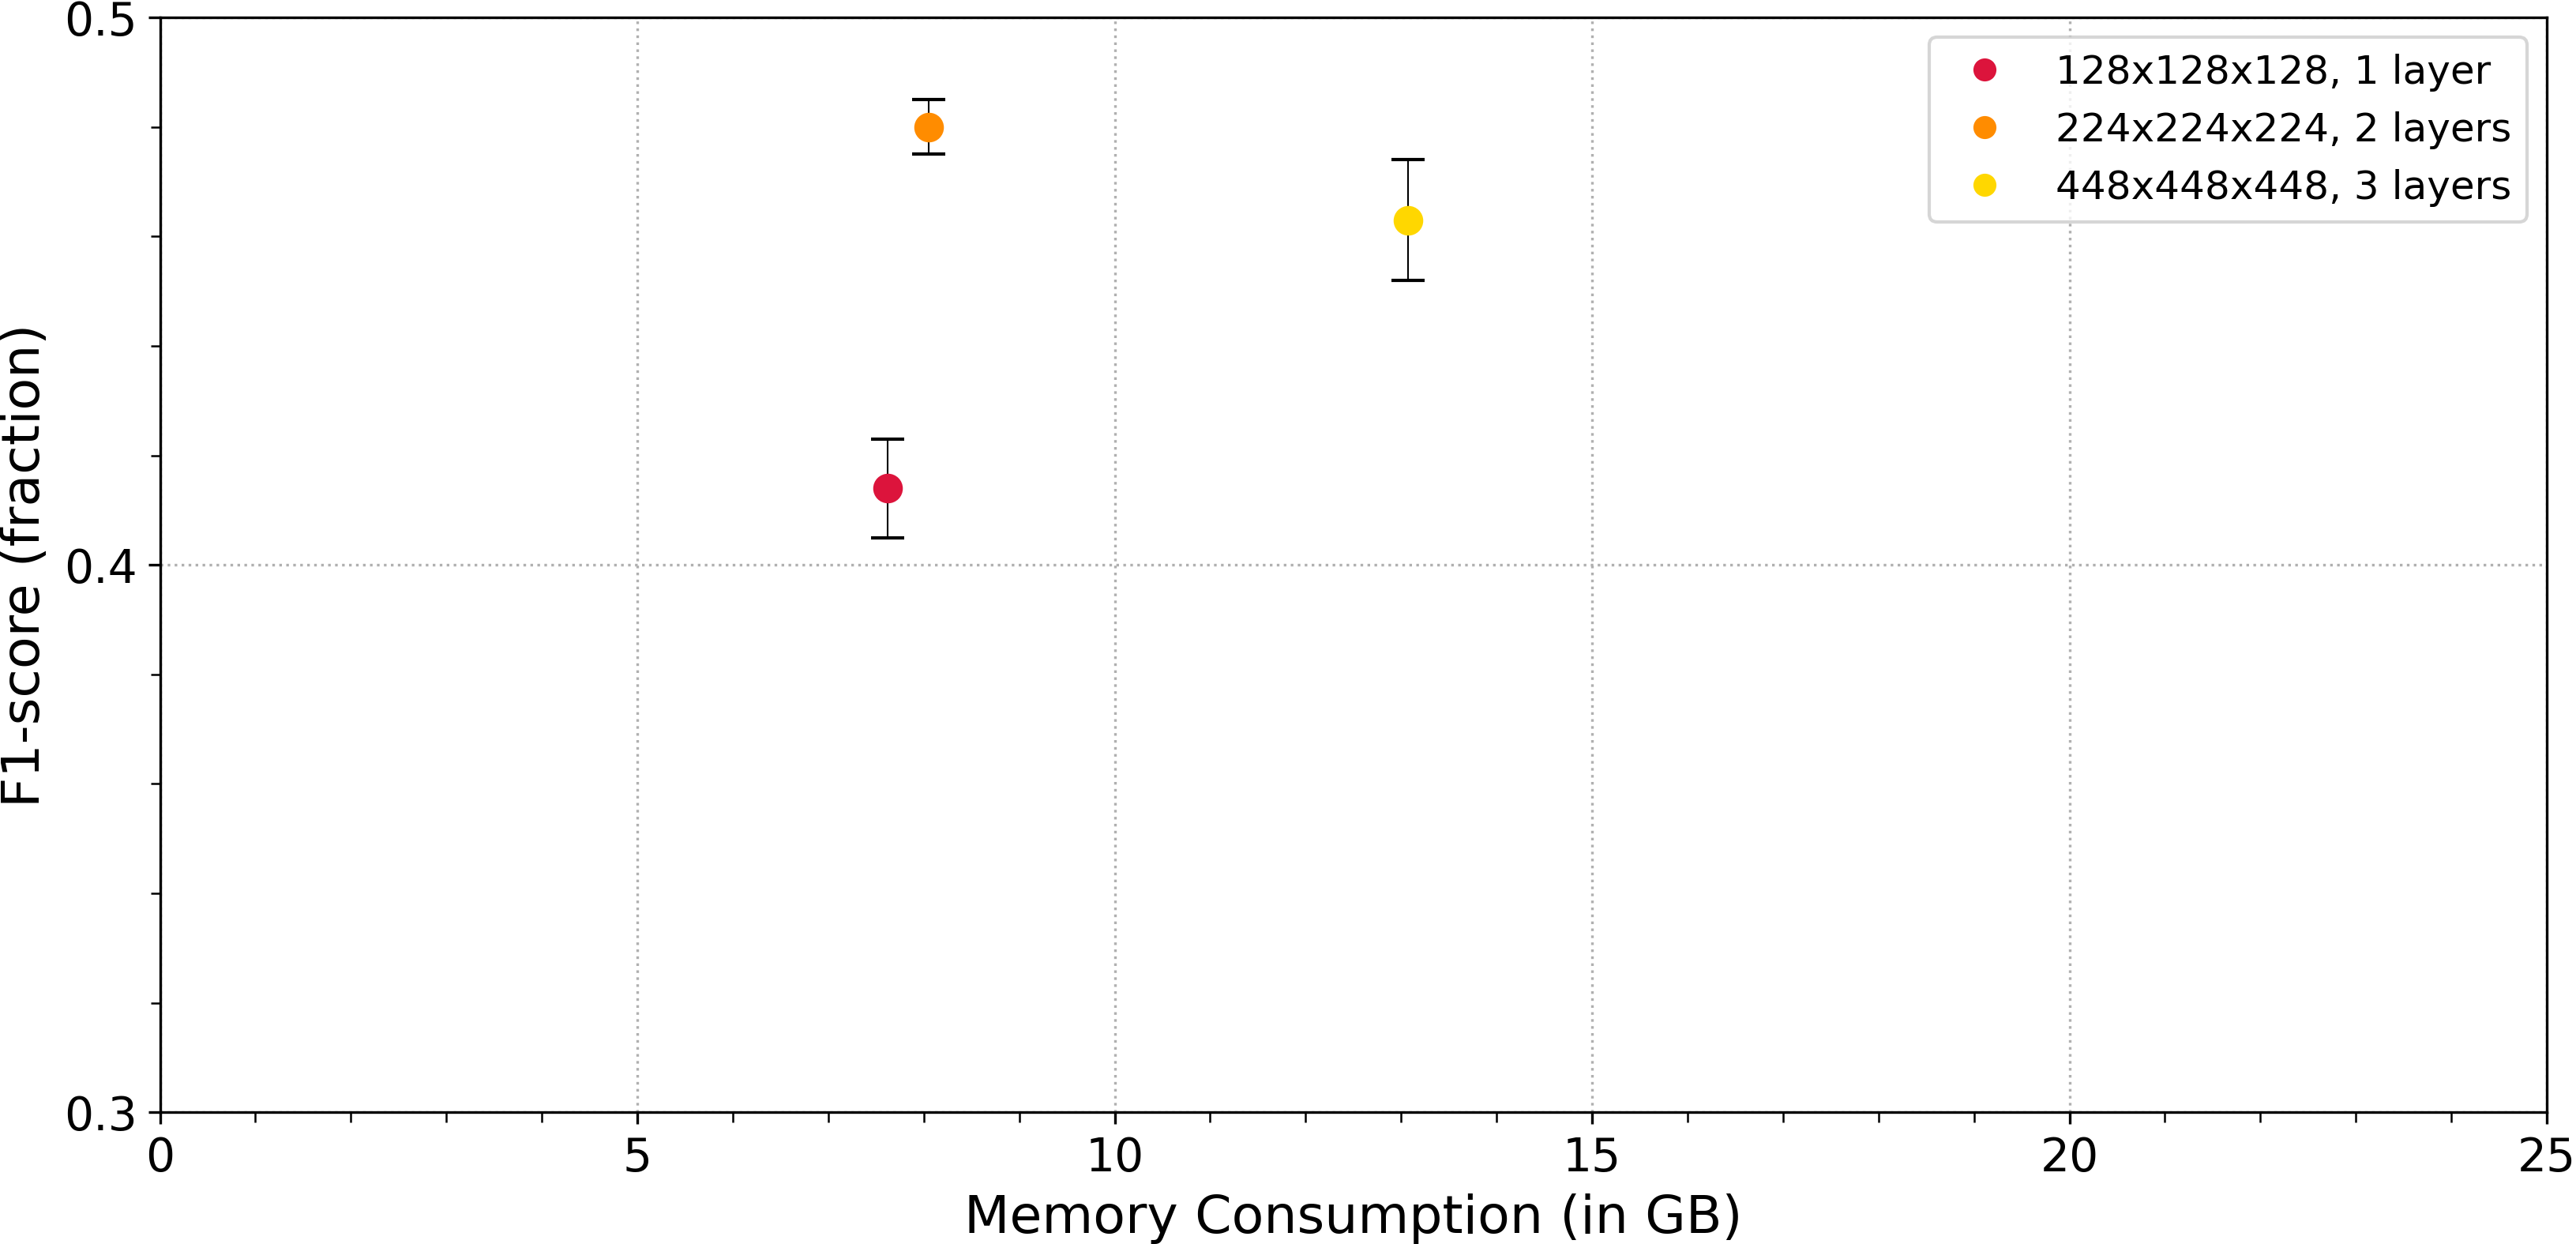
\includegraphics[width=1.0\textwidth]{./images/F1_vs_layers_memory.png}
	\caption[F1-score versus GPU memory consumption for different numbers of conv.~layers]{F1-score versus GPU memory consumption for different numbers of convolutional layers and volume sizes, keeping segmentation volume the same. The experiment with 4 convolutional layers was not executed due to very high memory demand.}
	\label{iou_vs_layers_memory}
\end{figure}
Interestingly, the configuration with two convolutional layers outperforms the one with three layers, which was not anticipated. The three-layer configuration's results, however, show a notably larger error bar compared to the others, indicating higher variance between runs. This suggests that the observed trend may not be reliable. Additional training runs could help to reduce the variance and provide more conclusive evidence regarding the optimal number of convolutional layers.



\section{Effects of Kernel Size on F1-score and Memory}
This experiment was conducted to examine the impact of the kernel size used in the central self-attention block on segmentation performance. The kernel size determines the spatial extent over which attention is applied and thus influences the model's ability to capture contextual information. Kernel sizes of 1, 3, 5, and 7 were evaluated for the standard  \gls{shvit}-SegFormer B5/S2-model with central self-attention and 2 convolution layers and an input size of {\tt (224,224,224)}, and the corresponding results illustrating the relationship between F1-score and \acrshort{gpu} memory usage are shown in figure \ref{iou_vs_kernel_memory}. 
\begin{figure}[H]
	\centering
	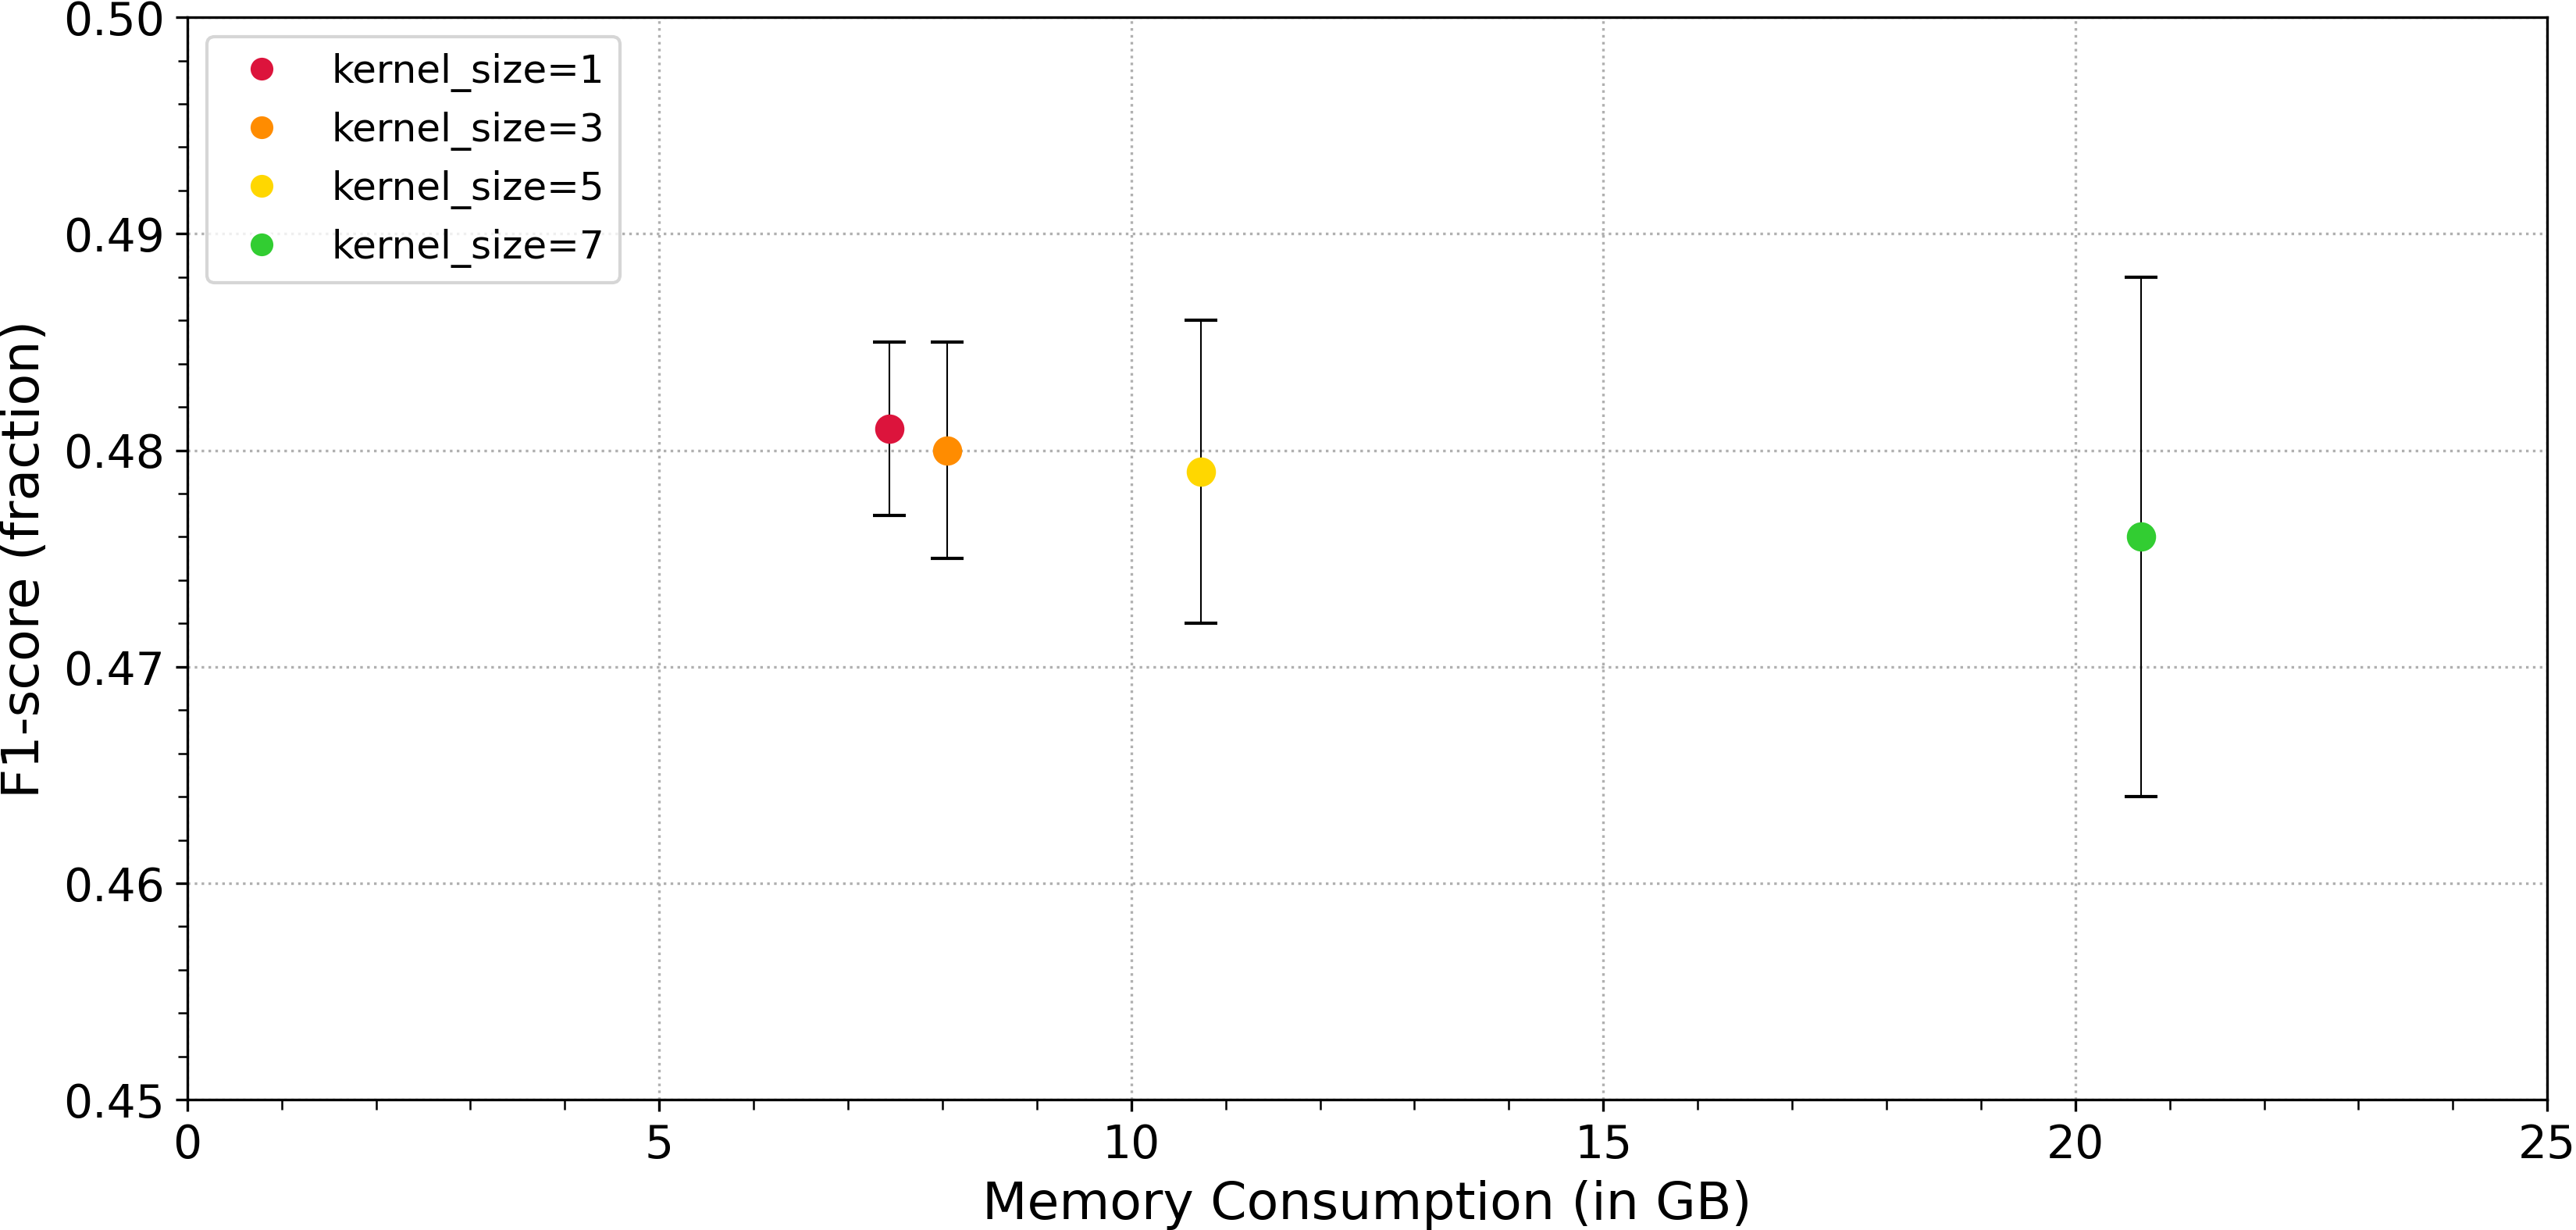
\includegraphics[width=1.0\textwidth]{./images/F1_vs_kernel_memory.png}
	\caption[F1-score versus GPU memory consumption for different kernel sizes]{F1-score versus GPU memory consumption for different kernel sizes.}
	\label{iou_vs_kernel_memory}
\end{figure}
A clear trend can be observed: the F1-score gradually decreases from {\tt kernel\_size=1} to {\tt kernel\_size=7}, with the error bar for {\tt kernel\_size=7} being noticeably larger than for other sizes. However, since the error bars overlap, it is difficult to confidently determine a statistically significant winner based solely on performance metrics. While {\tt kernel\_size=1} achieved the highest F1-score, followed closely by {\tt kernel\_size=3}, the marginal improvement with $1 \times 1$ kernels does not justify the loss of spatial modeling capability inherent in $3 \times 3$ kernels. Literature suggests that spatial context awareness enhances generalization performance, especially to unseen data, through the learning of spatially-coherent features rather than point-wise transformations \cite{he2015deepresiduallearningimage, simonyan2015deepconvolutionalnetworkslargescale, chollet2017xception}. In addition, training time per epoch increases substantially with larger kernels, rising from approximately 13 seconds for {\tt kernel\_size=1} to 51 seconds for {\tt kernel\_size=5}, and reaching 415 seconds for {\tt kernel\_size=7}. Considering both performance trends and the importance of spatial modeling capability, this study adopts {\tt kernel\_size=3} as the optimal configuration and recommends this setting for future experiments.

\medskip

In conclusion, these results showed that smaller attention kernel sizes led to higher F1-score than larger ones, a result which was not expected at first. However, literature suggests that smaller local attention windows are better at capturing fine structural details, which is especially important in \gls{3d} (medical) segmentation tasks. Studies such as \cite{Huang_2024, wu2024fewshotmedicalimagesegmentation, app142311365} support this hypothesis by showing that small-window attention helps preserve local texture and boundary precision, often leading to improved segmentation accuracy. These findings, well-established for convolutional kernels, suggest that attention mechanisms may benefit similarly from smaller kernel sizes, providing a theoretical foundation for the observed experimental results.

\medskip

As explained in section \ref{Transformer_Attention_Mechanisms}, the \gls{shcsa} block processes volumes of size {\tt (28,28,28)}, which are already relatively small. In this context, larger kernel sizes are less effective at capturing fine details.




\section[3D SHViT Segformer versus Residual SE UNet]{Segmentation performance: 3D SHViT Segformer versus Residual Squeeze and Excitation (SE) UNet}
To evaluate the segmentation performance and validate the \gls{3d} \gls{shvit} Segformer model, four distinct experiments were carried out. These experiments enabled a side-by-side comparison between the Residual Squeeze and Excitation (SE) UNet \cite{contribution_martin_leipert} and the \gls{shvit} Segformer architecture across different segmentation tasks. Performance evaluation is based on the F1-score calculated for individual semantic segments.

\medskip

This comparative analysis will provide insights into the relative strengths and limitations of convolutional versus transformer-based approaches for semantic segmentation tasks. To ensure a fair and direct comparison, both models use identical input specifications with volumetric data of {\tt (256,256,256)} voxels. The \gls{shvit} model is configured with hyperparameter settings of B5/S2 with central self-attention, and {\tt kernel\_size=3}, representing a balanced configuration between model complexity and computational efficiency. 


\subsection{Experiments 1-3: Comparative Analysis with Published Work}
The first three experiments were designed to replicate and compare \gls{3d} \gls{shvit} results with those reported in the existing literature \cite{contribution_martin_leipert}. These experiments serve as a benchmark to validate the implementation and ensure reproducibility of previously published findings. Each experiment follows the same methodology as the reference paper, enabling a direct performance comparison under identical conditions. The following tables summarize the obtained results.

\begin{center}
	\begin{threeparttable}[H]
		\begin{tabular}{lcc}
			\toprule[1.5pt]  
			& \multicolumn{2}{c}{Network} \\
			\multicolumn{1}{l}{F1-score} & {Residual SE UNet} & {SHViT Segformer} \\
			\midrule
			\midrule
			Total              & $0.821$ & $0.717 \pm 0.009$ \\
			\midrule
			Background         & $0.991$ & $0.958 \pm 0.002$ \\
			Shoe               & $0.882$ & $0.748 \pm 0.009$ \\
			Packaging Material & $0.589$ & $0.445 \pm 0.007$ \\
			\bottomrule
		\end{tabular}
		\captionsetup{width=0.95\textwidth}
		%		\captionsetup{width=\textwidth}
		\caption[Comparison of segmentation performance (F1-scores) between the Residual SE UNet and SHViT Segformer models across three different classes]{Experiment 1: Comparison of segmentation performance (F1-scores) between the Residual SE UNet and SHViT Segformer models across three different classes. The UNet model consistently outperforms SHViT Segformer, particularly for the \enquote{Shoe} and \enquote{Packaging Material} categories. Data for Residual SE UNet are taken from Table 2 \cite{contribution_martin_leipert}.}
		\label{tab:paper_3_segments}
	\end{threeparttable}
\end{center}

The results indicate that in all three comparative cases, the \gls{shvit} model demonstrates suboptimal performance in segmenting the defined segmentation classes, revealing challenges in the transformer-based approach for this specific application domain. Since the total F1-score is the averaged score of all segmentation classes, a poor result in one (or more) classes has a significant impact on the final score. 

\medskip 

Figure \ref{Paper_3Segments} shows the prediction results from the experiment using three segmentation classes, with images achieving high F1-scores displayed on the left and those with low F1-scores on the right.

\begin{figure}[H]
	\centering
	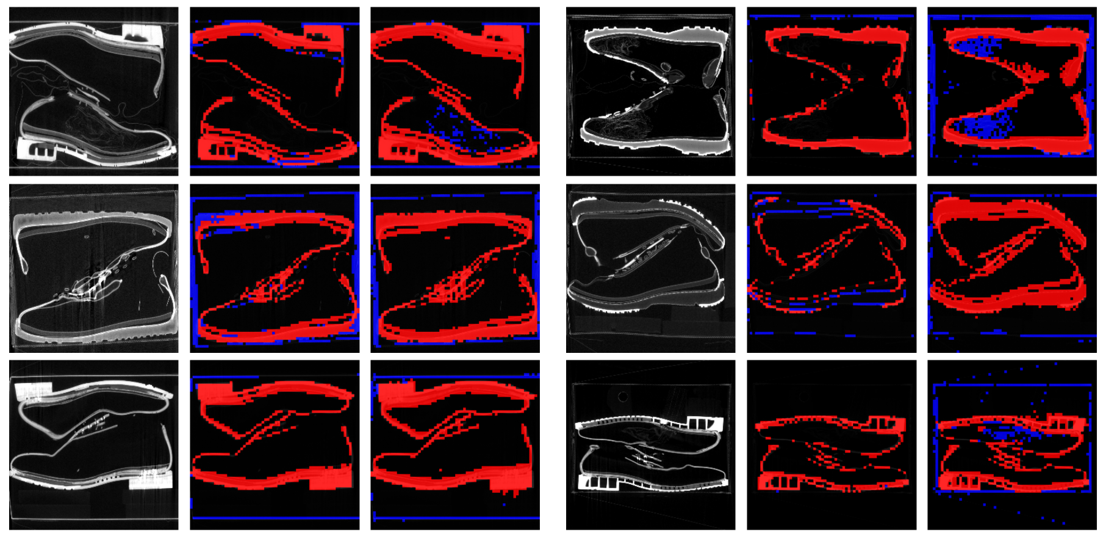
\includegraphics[width=1.0\textwidth]{./images/Paper_3Segments.png}
	
\includegraphics[width=0.9\textwidth]{./images/color_legend_3_classes.png}
	\caption[Results of shoes with 3 segments: background, shoe, and packaging material]{Results of shoes with 3 segments: background, shoe, and packaging material. From left to right: the input image, the predicted segmentation, and the corresponding ground truth segmentation image for each of the two columns. The images on the left have high overal F1-score ({\tt \small Bruschi\_down2\_2\_2: 0.829 [0.971, 0.840, 0.677]\footnotemark; Camper\_down2\_2\_2: 0.833 [0.948, 0.811, 0.740]; Herrenschuh\_43p5\_down2\_2\_2: 0.834 [0.968, 0.852, 0.682]}), the images on the right have a low F1-score ({\tt \small McKinley\_Anton\_down2\_2\_2: 0.620 [0.963, 0.750, 0.147]; Puma\_Silver\_down2\_2\_2: 0.659 [0.923, 0.487, 0.566]; Schuh\_Martin\_down2\_2\_2: 0.602 [0.977, 0.807, 0.023]}).}
	\label{Paper_3Segments}
\end{figure}
\footnotetext{{The order of these numbers are: total F1-score of the volume, in brackets the F1-score of background, shoe, and packaging material.}}

The background is detected with high confidence, typically achieving F1-scores well above 0.9 due to its large volume. The shoe is generally segmented well, while cardboard and packaging material show a higher standard deviation of nearly 0.2\footnote{The value of 0.2 should not be confused with the 0.007 in Table \ref{tab:paper_3_segments}. The latter is the standard deviation of mean values across five runs, while 0.2 reflects the deviation of packaging material across all volumes in the shoe dataset.}, likely because these relatively small regions are more difficult for the \gls{shvit} model to detect accurately.

\medskip

Experiments 2 and 3 use the same model architectures but modify the segmentation class definitions: experiment 2 simplifies the task to binary segmentation, while experiment 3 introduces four distinct classes.

\begin{center}
	\begin{threeparttable}[H]
		\begin{tabular}{lcc}
			\toprule[1.5pt]  
			& \multicolumn{2}{c}{Network} \\
			\multicolumn{1}{l}{F1-score} & {Residual SE UNet} & {SHViT Segformer} \\
			\midrule
			\midrule
			Total         & $0.902$ & $0.841 \pm 0.012$ \\
			\midrule
			Background    & $0.994$ & $0.980 \pm 0.002$ \\
			Inside Volume & $0.810$ & $0.701 \pm 0.023$ \\
			\bottomrule
		\end{tabular}
		\captionsetup{width=0.95\textwidth}
		%		\captionsetup{width=\textwidth}
		\caption[Comparison of segmentation performance (F1-scores) between the Residual SE UNet and SHViT Segformer models across two different classes]{Experiment 2: Comparison of segmentation performance (F1-scores) between the Residual SE UNet and SHViT Segformer models across two different classes. The UNet model achieves higher overall performance due to the better prediction of the \enquote{Inside Volume}. Data for Residual SE UNet are taken from Table 3 \cite{contribution_martin_leipert}.}
		\label{tab:paper_2_segments}
	\end{threeparttable}
\end{center}

\begin{figure}[H]
	\centering
	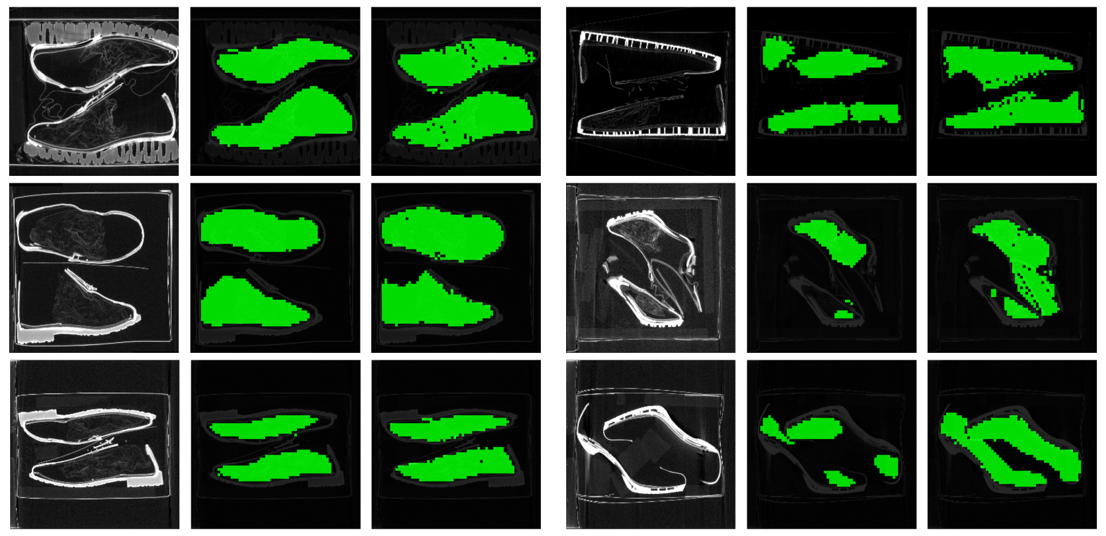
\includegraphics[width=1.0\textwidth]{./images/Paper_2Segments.png}
	
\includegraphics[width=0.9\textwidth]{./images/color_legend_2_classes.png}
	\caption[Results of shoes with 2 segments: background and inside volume]{Results of shoes with 2 segments: background and inside volume. From left to right: the input image, the predicted segmentation, and the corresponding ground truth segmentation image for each of the two columns. The images on the left have high overal F1-score ({\tt \small Shoepassion\_40\_down2\_2\_2: 0.936 [0.983, 0.889]\footnotemark; PetrolioSch-40-float\_down2\_2\_2: 0.919 [0.987, 0.852]; Petrolio-Sch-dunkelbraun\_44\_down2\_2\_2: 0.932 [0.995, 0.871]}), the images on the right have a low F1-score ({\tt \small Adidas\_Martin: 0.777 [0.983, 0.571]; Citywalk-sit-taupe-36\_down2\_2\_2: 0.713 [0.979, 0.447]; Tamaris-Pump-schwarz\_42\_down2\_2\_2: 0.755 [0.991, 0.519]}).}
	\label{Paper_2Segments}
\end{figure}
\footnotetext{{The order of these numbers are: total F1-score of the volume, in brackets the F1-score of background, and inside volume.}}

An analysis of the model's predictions using only two segments (background and inside volume) shows that the overall F1-score is very high. This is mainly due to the model's consistent ability to accurately identify the background, often achieving scores higher than 0.98. In contrast, the segmentation of the inside volume is less precise, leading to a lower F1-score for this class. This discrepancy highlights the challenge of identifying fine-grained features within the shoe, especially when visual cues are weak. The model appears to rely heavily on clear structural boundaries to segment the inside volume effectively. As a result, any ambiguity in shape or texture directly impacts performance. Improving the segmentation of the inside volume may therefore require more diverse training data or enhanced feature representations.

\medskip

A comparison between predictions with high and low scores indicates that the model performs well when the boundary of the sole and the upper material is clearly distinguishable, as can be seen in figure \ref{Paper_2Segments}. In such cases, the inside volume is segmented with high accuracy. However, when the boundary is unclear or contains open areas, as seen in the lower right image, the model often predicts the inside volume only at the tip and heel of the shoe, resulting in a reduced F1-score. This behavior suggests that the model struggles to generalize to less distinct input patterns, particularly in regions with missing or ambiguous boundary information.

\medskip

The results of experiment 3 are shown in table \ref{tab:paper_4_segments} and figure \ref{Paper_4Segments}:
\begin{center}
	\begin{threeparttable}[H]
		\begin{tabular}{lcc}
			\toprule[1.5pt]  
			& \multicolumn{2}{c}{Network} \\
			\multicolumn{1}{l}{F1-score} & {Residual SE UNet} & {SHViT Segformer} \\
			\midrule
			\midrule
			Total          & $0.873$ & $0.702 \pm 0.003$ \\
			\midrule
			Background     & $0.997$ & $0.984 \pm 0.000$ \\
			Outer Sole     & $0.887$ & $0.777 \pm 0.006$ \\
			Inner Sole     & $0.795$ & $0.459 \pm 0.012$ \\
			Upper Material & $0.813$ & $0.586 \pm 0.008$ \\
			\bottomrule
		\end{tabular}
		\captionsetup{width=0.95\textwidth}
		%		\captionsetup{width=\textwidth}
		\caption[Comparison of segmentation performance (F1-scores) between the Residual SE UNet and SHViT Segformer models across four different classes]{Experiment 3: Comparison of segmentation performance (F1-scores) between the Residual SE UNet and SHViT Segformer models across four different classes. The F1-score of UNet model for the segments \enquote{Inner Sole} and \enquote{Upper Material} is higher than for the SHViT Segformer model. Data for Residual SE UNet are taken from Table 4 \cite{contribution_martin_leipert}.}
		\label{tab:paper_4_segments}
	\end{threeparttable}
\end{center}

\begin{figure}[H]
	\centering
	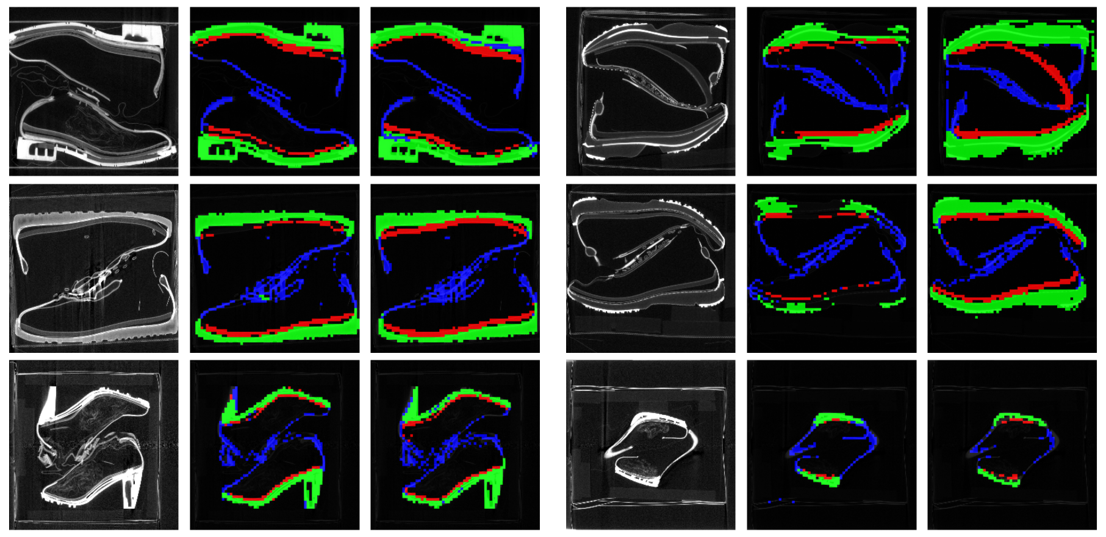
\includegraphics[width=1.0\textwidth]{./images/Paper_4Segments.png}
	
\includegraphics[width=0.8\textwidth]{./images/color_legend_4_classes.png}
	\caption[Results of shoes with 4 segments: background, outer and inner sole, and upper material]{Results of shoes with 4 segments: background, outer sole, inner sole, and upper material. From left to right: the input image, the predicted segmentation, and the corresponding ground truth segmentation image for each of the two columns. The images on the left have high overal F1-score ({\tt \small Bruschi\_down2\_2\_2: 0.764 [0.982, 0.811, 0.605, 0.660]\footnotemark; Camper\_down2\_2\_2: 0.777 [0.971, 0.875, 0.550, 0.711]; Citywalk-sit-taupe-39\_down2\_2\_2: 0.768 [0.994, 0.840, 0.598, 0.641]}), the images on the right have a low F1-score ({\tt \small Puma\_38\_down2\_2\_2: 0.645 [0.940, 0.631, 0.386, 0.624]; Puma\_Silver\_down2\_2\_2:  0.580 [0.948, 0.431, 0.353, 0.589]; Tamaris-Pump-Schwarz-38\_down2\_2\_2: 0.643 [0.995, 0.665, 0.513, 0.400]}).}
	\label{Paper_4Segments}
\end{figure}
\footnotetext{{The order of these numbers are: total F1-score of the volume, in brackets the F1-score of background, outer sole, inner sole, and upper material.}}

Analyzing the standard deviation of the predictions for the 40 shoes reveals the class that is most difficult to predict. In this case, the thin layer of the inner sole shows the highest standard deviation of 0.11, indicating a substantial variation between accurate and less accurate predictions. The outer sole and upper material follow, each with a standard deviation of approximately 0.08. In contrast, the background exhibits a low deviation, indicating more consistent predictions for this class. The green area shown in the two images in the upper right represents the outer sole of the shoe. The model encounters difficulties, visible as unfilled gaps in the image, when the bright line of the outer sole suddenly changes from light to dark. In contrast, no such issues occur when the outer sole is depicted with consistent brightness.

\medskip

It was also observed that the model can produce a visually good prediction while still achieving a low F1-score. This can be seen, for example, in the bottom right image when comparing the predicted image with the ground truth. It is noticeable that in the ground truth image, the upper material (blue color) is not fully represented. Since the F1-score is calculated by comparing the prediction with the ground truth, discrepancies between the two inevitably lead to a lower score, even though the prediction itself is actually of good quality.

\bigskip

The experimental results summarized in tables \ref{tab:paper_3_segments} to \ref{tab:paper_4_segments} show that \gls{shvit} performs not as well as UNet-\gls{cnn}. A literature review offers more details about this performance gap.

\medskip

Convolutional networks like the Residual SE UNet generally outperform transformer-based models such as \gls{shvit} Segformer in semantic segmentation tasks, especially on small datasets. One of the main reasons is that \glspl{cnn} have a strong inductive bias \cite{Dosovitskiy2021ViT}. They are designed to recognize local patterns like edges and textures, which helps them generalize well even from limited data. In contrast, Vision Transformers lack this bias and need much more training data to learn spatial relationships effectively \cite{ronneberger2015, steiner2022trainvitdataaugmentation}.

\medskip

Moreover, \glspl{cnn} like UNet use skip connections that preserve high-resolution features, which is especially important for accurately segmenting small or fine-grained objects (e.g., shoe tongues or packaging material) \cite{zhou2018unet}. Transformers, when trained from scratch, tend to produce coarser outputs and have problems capturing such details. This implies that without large datasets or pretrained weights, \glspl{vit} struggle to capture fine structure, which supports the claim of coarser outputs and weaker detail segmentation. As a result, the UNet model performs more robustly in data-scarce, detail-sensitive segmentation scenarios \cite{steiner2022trainvitdataaugmentation}.


{\subsection[Experiment 4: Standard 3D SHViT Segformer Model Evaluation]{Experiment 4: Standard 3D SHViT Segformer Model \\ Eva\-luation}
The fourth experiment uses a standard \gls{3d} \gls{shvit} model configuration to establish baseline performance metrics for the transformer-based segmentation approach. This experiment provides a reference point for evaluating the effectiveness of the hierarchical vision transformer architecture in the specific application domain.

\begin{center}
	\begin{threeparttable}[H]
		\begin{tabular}{lcc}
			\toprule[1.5pt]  
			& \multicolumn{1}{c}{Network} \\
			\multicolumn{1}{l}{F1-score} & {SHViT Segformer} \\
			\midrule
			\midrule
			Total              & $0.485 \pm 0.009$ \\
			\midrule
			Background         & $0.950 \pm 0.009$ \\
			Box                & $0.442 \pm 0.024$ \\
			Inner Sole         & $0.462 \pm 0.010$ \\
			Outer Sole         & $0.742 \pm 0.009$ \\
			Upper Material     & $0.522 \pm 0.006$ \\
			Tongue/Flap        & $0.156 \pm 0.028$ \\
			Packaging Material & $0.120 \pm 0.013$ \\
			\bottomrule
		\end{tabular}
		\captionsetup{width=0.95\textwidth}
		%		\captionsetup{width=\textwidth}
		\caption[Segmentation performance (F1-scores) of the SHViT Segformer across seven classes]{Experiment 4: Segmentation performance (F1-scores) of the SHViT Segformer across seven classes. Results for the Residual SE UNet are not available for this experimental setup. The model performs well on large structures like \enquote{Background} and \enquote{Outer Sole}, but has problems with fine-grained regions such as \enquote{Packaging Material} and \enquote{Tongue / Flap}.}
		\label{tab:paper_7_segments}
	\end{threeparttable}
\end{center}

Small objects or specific components such as the shoe tongue or packaging material exhibit poor segmentation performance, resulting in significantly low F1-scores for these classes. This poor performance in segmenting fine-detailed or smaller features has a substantial impact on the overall F1-score of the model, as these classes contribute disproportionately to the averaged total score. Results\footnote{The results shown in Figure \ref{result_for_shvit_with_center_attention} were generated using a resolution of {\tt (224,224,224)}, but there is little noticeable difference compared to images with an edge length of 256 pixels.} of can be found in figure \ref{result_for_shvit_with_center_attention} on page \pageref{result_for_shvit_with_center_attention}.

\medskip

It is important to note that the current results were obtained using only 40 pairs of shoes, split for training in a 5-fold cross-validation setup with data augmentation. Given the limited size of the dataset, these results should be considered as a baseline, providing a foundation for further investigations or improvements through larger datasets, refined annotations, or more advanced model architectures.



\section{Recommended Model Configuration}
Based on the investigations conducted and discussed in the preceding sections of this chapter, the following conclusions have been drawn and corresponding recommendations are provided: The model achieving the highest F1-accuracy, along with the most favorable accuracy-to-memory trade-off, is the \gls{3d} \gls{shvit}-SegFormer with central self-attention configured with the B5/S2 parametrization\footnote{see also table \ref{tab:variants} in section \ref{sec:Architecture_of_SHViT_Segformer} on page \pageref{sec:Architecture_of_SHViT_Segformer}} and two convolutional heads in the \gls{shvit} encoder head. The kernel size of the central self-attention layer is 3 due to its F1-score with low deviation. It achieves for an input volume of {\tt (224,224,224)} an F1 of $0.480 \pm 0.005$, with a memory consumption of 8.05\,GB and a training time of around 13 seconds per epoch. With this configuration input volumes up to {\tt (320,320,320)} are possible.
